\documentclass[a4paper,11pt]{article}
%\documentclass[a4paper,twoside,11pt,titlepage]{book}
\usepackage{listings}
\usepackage[utf8]{inputenc}
\usepackage[spanish]{babel}
\usepackage{cite}
\usepackage{eurosym}
\usepackage{algpseudocode}
\usepackage{float}
\usepackage{rotating}
\usepackage{fancyhdr}

% \usepackage[style=list, number=none]{glossary} %
%\usepackage{titlesec}
%\usepackage{pailatino}

\decimalpoint
\usepackage{dcolumn}
\newcolumntype{.}{D{.}{\esperiod}{-1}}
\makeatletter
\addto\shorthandsspanish{\let\esperiod\es@period@code}
\makeatother


%\usepackage[chapter]{algorithm}
\RequirePackage{verbatim}
%\RequirePackage[Glenn]{fncychap}

\usepackage{graphicx}
\usepackage{afterpage}

\usepackage{longtable}

\usepackage[pdfborder={000}]{hyperref} %referencia

% ********************************************************************
% Re-usable information
% ********************************************************************
\newcommand{\myTitle}{Implementación de tareas de manipulación precisa con brazos robóticos\xspace}
\newcommand{\myDegree}{Grado en Ingeniería Informática\xspace}
\newcommand{\myName}{Cristina María Garrido López\xspace}
\newcommand{\myProf}{Eduardo Ros Vidal\xspace}
\newcommand{\myOtherProf}{Francisco Barranco Expósito\xspace}
%\newcommand{\mySupervisor}{Put name here\xspace}
\newcommand{\myFaculty}{Escuela Técnica Superior de Ingenierías Informática y de
Telecomunicación\xspace}
\newcommand{\myFacultyShort}{E.T.S. de Ingenierías Informática y de
Telecomunicación\xspace}
\newcommand{\myDepartment}{Departamento de Arquitectura y Tecnología de Computadores\xspace}
\newcommand{\myUni}{\protect{Universidad de Granada}\xspace}
\newcommand{\myLocation}{Granada\xspace}
\newcommand{\myTime}{\today\xspace}
\newcommand{\myVersion}{Version 0.1\xspace}

\hypersetup{
	colorlinks,
	citecolor=black,
	filecolor=black,
	linkcolor=black,
	urlcolor=black
}

\hypersetup{
pdfauthor = {\myName (email (en) ugr (punto) es)},
pdftitle = {\myTitle},
pdfsubject = {},
pdfkeywords = {palabra_clave1, palabra_clave2, palabra_clave3, ...},
pdfcreator = {LaTeX con el paquete ....},
pdfproducer = {pdflatex}
}

%\hyphenation{}


%\usepackage{doxygen/doxygen}
%\usepackage{pdfpages}
\usepackage{url}
\usepackage{colortbl,longtable}
\usepackage[stable]{footmisc}
%\usepackage{index}

%\makeindex
%\usepackage[style=long, cols=2,border=plain,toc=true,number=none]{glossary}
% \makeglossary

% Definición de comandos que me son tiles:
%\renewcommand{\indexname}{Índice alfabético}
%\renewcommand{\glossaryname}{Glosario}

\pagestyle{fancy}
\fancyhf{}



%\renewcommand{\chaptermark}[1]{\markboth{\textbf{#1}}{}}
\renewcommand{\sectionmark}[1]{\markright{\textbf{\thesection. #1}}}

\setlength{\headheight}{1.5\headheight}

\newcommand{\HRule}{\rule{\linewidth}{0.5mm}}
%Definimos los tipos teorema, ejemplo y definición podremos usar estos tipos
%simplemente poniendo \begin{teorema} \end{teorema} ...
%\newtheorem{teorema}{Teorema}[chapter]
%\newtheorem{ejemplo}{Ejemplo}[chapter]
%\newtheorem{definicion}{Definición}[chapter]

\definecolor{gray97}{gray}{.97}
\definecolor{gray75}{gray}{.75}
\definecolor{gray45}{gray}{.45}
\definecolor{gray30}{gray}{.94}

\lstset{ frame=Ltb,
     framerule=0.5pt,
     aboveskip=0.5cm,
     framextopmargin=3pt,
     framexbottommargin=3pt,
     framexleftmargin=0.1cm,
     framesep=0pt,
     rulesep=.4pt,
     backgroundcolor=\color{gray97},
     rulesepcolor=\color{black},
     %
     stringstyle=\ttfamily,
     showstringspaces = false,
     basicstyle=\scriptsize\ttfamily,
     commentstyle=\color{gray45},
     keywordstyle=\bfseries,
     %
     numbers=left,
     numbersep=6pt,
     numberstyle=\tiny,
     numberfirstline = false,
     breaklines=true,
   }
 
% minimizar fragmentado de listados
\lstnewenvironment{listing}[1][]
   {\lstset{#1}\pagebreak[0]}{\pagebreak[0]}

\lstdefinestyle{CodigoC}
   {
	basicstyle=\scriptsize,
	frame=single,
	language=C,
	numbers=left
   }
\lstdefinestyle{CodigoC++}
   {
	basicstyle=\small,
	frame=single,
	backgroundcolor=\color{gray30},
	language=C++,
	numbers=left
   }

 
\lstdefinestyle{Consola}
   {basicstyle=\scriptsize\bf\ttfamily,
    backgroundcolor=\color{gray30},
    frame=single,
    numbers=none
   }


\newcommand{\bigrule}{\titlerule[0.5mm]}


%Para conseguir que en las páginas en blanco no ponga cabecerass
\makeatletter
\def\clearpage{%
  \ifvmode
    \ifnum \@dbltopnum =\m@ne
      \ifdim \pagetotal <\topskip
        \hbox{}
      \fi
    \fi
  \fi
  \newpage
  \thispagestyle{empty}
  \write\m@ne{}
  \vbox{}
  \penalty -\@Mi
}
\makeatother

\usepackage{pdfpages}
\begin{document}
\begin{titlepage}
 
 
\newlength{\centeroffset}
\setlength{\centeroffset}{-0.5\oddsidemargin}
\addtolength{\centeroffset}{0.5\evensidemargin}
\thispagestyle{empty}

\noindent\hspace*{\centeroffset}\begin{minipage}{\textwidth}

\centering

\includegraphics[width=0.9\textwidth]{imagenes/logo_ugr.jpg}\\[1.4cm]

\textsc{ \Large TRABAJO FIN DE GRADO\\[0.2cm]}
\textsc{ INGENIERÍA EN INFORMÁTICA}\\[1cm]
% Upper part of the page
% 
% Title
{\Huge\bfseries Implementación de tareas de manipulación precisa con brazos robóticos\\
}
\noindent\rule[-1ex]{\textwidth}{3pt}\\[3.5ex]
{\large\bfseries }
\end{minipage}

\vspace{1.5cm}
\noindent\hspace*{\centeroffset}\begin{minipage}{\textwidth}
\centering

\textbf{Autor}\\ {Cristina María Garrido López}\\[2.5ex]
\textbf{Directores}\\
{Eduardo Ros Vidal\\
Francisco Barranco Expósito}\\[2cm]

\includegraphics[width=0.3\textwidth]{imagenes/etsiit_logo.png}\\[0.1cm]
\textsc{Escuela Técnica Superior de Ingenierías Informática y de Telecomunicación}\\
\textsc{---}\\
\date{\today}
Granada, a 18 de Junio de 2018 
\end{minipage}
%\addtolength{\textwidth}{\centeroffset}
%\vspace{\stretch{2}}
\end{titlepage}



\chapter*{}
%\thispagestyle{empty}
%\cleardoublepage

%\thispagestyle{empty}

%\begin{titlepage}
 
 
\setlength{\centeroffset}{-0.5\oddsidemargin}
\addtolength{\centeroffset}{0.5\evensidemargin}
\thispagestyle{empty}

\noindent\hspace*{\centeroffset}\begin{minipage}{\textwidth}

\centering
%
\includegraphics[width=0.9\textwidth]{imagenes/logo_ugr.jpg}\\[1.4cm]

%\textsc{ \Large PROYECTO FIN DE CARRERA\\[0.2cm]}
%\textsc{ INGENIERÍA EN INFORMÁTICA}\\[1cm]
% Upper part of the page
% 

 \vspace{3.3cm}

%si el proyecto tiene logo poner aquí

\includegraphics{imagenes/logo.png} 
 \vspace{0.5cm}

% Title

{\Huge\bfseries Título del proyecto\\
}
\noindent\rule[-1ex]{\textwidth}{3pt}\\[3.5ex]
{\large\bfseries Subtítulo del proyecto.\\[4cm]}
\end{minipage}

\vspace{2.5cm}
\noindent\hspace*{\centeroffset}\begin{minipage}{\textwidth}
\centering

\textbf{Autor}\\ {Nombre Apellido1 Apellido2 (alumno)}\\[2.5ex]
\textbf{Directores}\\
{Nombre Apellido1 Apellido2 (tutor1)\\
Nombre Apellido1 Apellido2 (tutor2)}\\[2cm]
%
\includegraphics[width=0.15\textwidth]{imagenes/tstc.png}\\[0.1cm]
%\textsc{Departamento de Teoría de la Señal, Telemática y Comunicaciones}\\
%\textsc{---}\\
%Granada, mes de 201
\end{minipage}
%\addtolength{\textwidth}{\centeroffset}
\vspace{\stretch{2}}

 
\end{titlepage}






\cleardoublepage
\thispagestyle{empty}

\begin{center}
{\large\bfseries Implementación de tareas de manipulación precisa con brazos robóticos}\\
\end{center}
\begin{center}
Cristina María Garrido López\\
\end{center}

%\vspace{0.7cm}
\noindent{\textbf{Palabras clave}: robótica, clasificación, clustering, k-medias, planificación de trayectorias, filtrado por color.}\\

\vspace{0.7cm}
\noindent{\textbf{Resumen}}\\

\noindent Este proyecto final de grado presenta el desarrollo de tareas de manipulación de objetos y evaluación de prestaciones, así como análisis de eficiencia de cada algoritmo programado. Se utiliza el robot Baxter de Rethink Robotics y el sistema operativo de robots (ROS). \\

\noindent Se fija como objetivo principal la automatización de tareas de clasificación de objetos en distintos entornos utilizando uno de los brazos robóticos de Baxter para realizar los procesos de visión y control. Posteriormente, se realizarán comparaciones con distinto tamaño y número de objetos en los diferentes entornos.\\

\noindent Se explicarán las funcionalidades del framework ROS, MoveIt! y los componentes hardware de Baxter, así como los métodos utilizados de visión por computador. \\

\noindent Puesto que es difícil encontrar código abierto en robótica, los algoritmos desarrollados en este proyecto serán liberados de forma que puedan ser utilizados por otros investigadores, esperando que así sea más útil para la comunidad.\\
%\noindent El contenido de este proyecto se encuentra disponible en
\cleardoublepage


\thispagestyle{empty}


\begin{center}
{\large\bfseries Precise handling tasks implementation with robotic arms}\\
\end{center}
\begin{center}
Cristina María Garrido López\\
\end{center}

%\vspace{0.7cm}
\noindent{\textbf{Keywords}: Robotics, classification, clustering, k-means, trajectory planning, colour filter.}\\

\vspace{0.7cm}
\noindent{\textbf{Abstract}}\\

\noindent This Bachelor thesis presents the development of various manipulation tasks and performance evaluation, where the Baxter Robot from Rethink Robotics and the Robot Operating System (ROS) are used. \\

\noindent The main objective is to automate object classification tasks in different environments, using one of Baxter's two robotic arms to carry out computer vision tasks and operational level control. Later, tests will be made with different size and number of objets in the different environments. \\

\noindent ROS functionalities, MoveIt! and Baxter's hardware components will be explained, as well as the computer vision methods. \\

\noindent Since it is difficult to find open source in the field of robotics, the developed algorithms in this thesis will be released so that they can be used by other researchers, hoping it is useful for the comunity. \\

\chapter*{}
\newpage
\thispagestyle{empty}

\noindent\rule[-1ex]{\textwidth}{2pt}\\[4.5ex]

Yo, \textbf{Cristina María Garrido López}, alumna de la titulación Ingeniería en Informática de la \textbf{Escuela Técnica Superior
de Ingenierías Informática y de Telecomunicación de la Universidad de Granada}, con DNI *, autorizo la
ubicación de la siguiente copia de mi Trabajo Fin de Grado en la biblioteca del centro para que pueda ser
consultada por las personas que lo deseen.

\vspace{6cm}

\noindent Fdo: Cristina María Garrido López

\vspace{2cm}

\begin{flushright}
Granada a 17 de Junio de 2018.
\end{flushright}

\newpage
\chapter*{}
\thispagestyle{empty}

\noindent\rule[-1ex]{\textwidth}{2pt}\\[4.5ex]

D. \textbf{Eduardo Ros Vidal}, Profesor del Área de Arquitectura y Tecnología de Computadores del Departamento de Arquitectura y Tecnología de Computadores de la Universidad de Granada.

\vspace{0.5cm}

D. \textbf{Francisco Barranco Expósito}, Profesor del Área de Arquitectura y Tecnología de Computadores del Departamento de Arquitectura y Tecnología de Computadores de la Universidad de Granada.


\vspace{0.5cm}

\textbf{Informan:}

\vspace{0.5cm}

Que el presente trabajo, titulado \textit{\textbf{Implementación de tareas de manipulación precisa con brazos robóticos}},
ha sido realizado bajo su supervisión por \textbf{Cristina María Garrido López}, y autorizamos la defensa de dicho trabajo ante el tribunal
que corresponda.

\vspace{0.5cm}

Y para que conste, expiden y firman el presente informe en Granada a 18 de Junio de 2018.

\vspace{1cm}

\textbf{Los directores:}

\vspace{5cm}

\noindent \textbf{Eduardo Ros Vidal \ \ \ \ \ \ \ \ \ \ \ \ \ \ \ \ \ \ \ Francisco Barranco Expósito}

\newpage
\section*{Agradecimientos}
\thispagestyle{empty}

       \vspace{1cm}


\noindent Sobre todo, me gustaría agradecer todo el apoyo, tiempo invertido y consejo proporcionado por los tutores de este proyecto, Eduardo Ros y Francisco Barranco, que nunca han faltado cuando he necesitado su ayuda. Por supuesto, agradezco además el hecho de permitirme trabajar en el laboratorio del CITIC y aportarme los materiales necesarios para realizar mi proyecto. \\

\noindent También me gustaría expresar mi gratitud hacia mis amigos de la facultad, a mi familia y a mis amigas por todo el apoyo durante el curso.\\


\newpage
\section*{Declaración de autoría y originalidad del TFG}

\vspace{1cm}

\noindent Yo, Cristina María Garrido López, con DNI *, declaro que el presente documento ha sido realizado por mí y se basa en mi propio trabajo, a menos que se indique lo contrario. No se ha utilizado el trabajo de ninguna otra persona sin el debido reconocimiento. Todas las referencias han sido citadas y todas las fuentes de información y conjuntos de datos han sido específicamente reconocidos. \\

\vspace{6cm}

\noindent Fdo: Cristina María Garrido López

\vspace{2cm}

\begin{flushright}
	Granada a 17 de Junio de 2018.
\end{flushright}

\newpage
%\frontmatter
\tableofcontents
\newpage
\listoffigures
\newpage
\listoftables
\newpage
%

%\mainmatter
%\setlength{\parskip}{5pt}
\newpage
\section{Introducción}
\label{intro}
\noindent Para realizar este trabajo se ha utilizado a Baxter, un robot desarrollado por Rethink Robotics, como robot de investigación, encargado de realizar las diferentes tareas mostradas a lo largo del documento. \\

\noindent La automatización de procesos es cada vez más frecuente en la industria, es por ello que este tipo de robots seguros, que no necesitan de una infraestructura para aislarse de las personas, se utilizan. Además de la posibilidad de trabajar colaborando con un humano, son fáciles de programar, de desplazar y tienen un bajo coste comparado con el coste usual de los robots industriales.\\
Estos robots se pueden programar a través del entorno ROS, del cual se puede encontrar bastante documentación en internet, además de tener una gran comunidad, útil para consultar o solventar cualquier duda existente. \\

\begin{figure}[H]
	\centering % si queremos la imagen centrada
	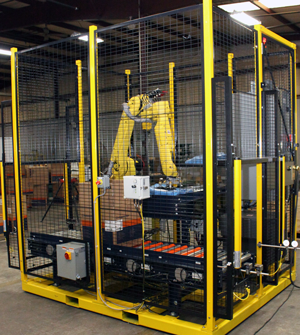
\includegraphics[scale=0.6]{imagenes/cage.png}
	\caption{Brazo robótico aislado}
\end{figure}

\noindent Como se ve en la siguiente imagen (obtenida de \cite{robgraph}), se espera que el mercado de robots industriales crezca considerablemente en los próximos años. Algunas fuentes indican que este crecimiento puede llegar a ser exponencial, llegando a aumentar de 16850 millones de dólares en 2017 a 48170 millones en 2025 \cite{robmark}. \\

\begin{figure}[H]
	\centering % si queremos la imagen centrada
	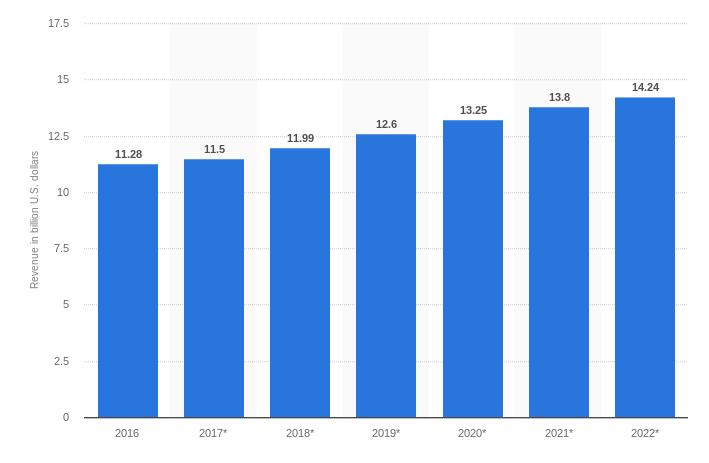
\includegraphics[scale=0.5]{imagenes/robmarket.jpg}
	\caption{Gráfica que muestra el crecimiento del mercado de robots industriales\cite{robgraph}. El eje horizontal representa el año y el eje vertical miles de millones de dólares}
\end{figure}

\noindent En este documento se explicarán las plataformas software y hardware utilizadas para realizar las tareas de clasificación de objetos con Baxter, en entorno estático y dinámico, además de realizar una comparativa de eficiencia con distintos parámetros. \\

\subsection{Motivación}
\noindent A día de hoy, en la industria existen muchos trabajos realizados por personas, a pesar de que pueden resultar peligrosos o dañinos para ellas \cite{lasota2014toward}. Debido a esto, la automatización de estas tareas resulta interesante, siendo realizadas por robots industriales que, en muchas ocasiones, suelen superar los 100000 euros.\\

\noindent En este proyecto se ha utilizado a Baxter, un robot desarrollado por Rethink Robotics, menos costoso y más seguro \cite{ju2014kinematics}, simulando una cadena de producción en la que Baxter se encarga de clasificar los objetos por color y posición, empleando el framework ROS (Robotic Operating System), MoveIt! y RViz. \\

\subsection{Situación inicial}
\noindent Como ya se ha dicho, en este proyecto se pretende realizar una clasificación de objetos en entorno estático y dinámico. Se dispone de una cinta transportadora que se utilizará en las pruebas de entorno dinámico, del robot Baxter y de las plataformas MoveIt! y RViz. Para el desarrollo de los algoritmos, se parte de un filtro de color \cite{maik}, al que se le añadirán las funcionalidades de segmentación por color y posición, planificación y ejecución de trayectorias y se realizarán distintos programas encargados de controlar a Baxter para realizar la clasificación. \\


\subsection{Objetivos}
\label{objetivos}
\noindent En este trabajo se realiza un estudio de las prestaciones de Baxter en tareas que incluyen clasificación de objetos y visión por computador. Para ello han sido fijados los siguientes objetivos:
\begin{itemize}
	\item Estudio de las funcionalidades y servicios del framework ROS.
	\item Integración de un filtro de color que permita realizar la clasificación basada en esta característica, y cálculo de grupos de objetos segmentados y recta que los separa.
	\item Desarrollo de diversos programas de clasificación de objetos y \textit{pick and place}.
	\item Clasificación de objetos según un parámetro que especifica el porcentaje de objetos de un color a obtener.
	\item Robótica adaptativa. Con la misma configuración de objetos, el esquema de control adaptará un parámetro a partir del grado de éxito de la ejecución anterior en entorno estático, lo que proporcionará cierto grado de adaptación y optimización. Este parámetro modificará el valor del brazo en el eje de ordenadas.

	\item Realización de pruebas, estudio de prestaciones y barras de error de las tareas realizadas.
	\item Liberación del software desarrollado y documentación alojados en \textit{GitHub}. Creación de una web con el contenido para que pueda ser utilizado por otros investigadores.
\end{itemize}

\subsection{Procedimiento}
\noindent Estos objetivos se pueden englobar en dos módulos, \textbf{módulo de reconocimiento}, encargado de realizar la segmentación por color y posición y enviar los datos obtenidos al \textbf{módulo de control}, cuya función será controlar a Baxter para realizar los movimientos definidos por la planificación de trayectorias. \\
\noindent Así pues, puntualizamos varias funcionalidades:

\begin{itemize}
	\item Identificación de objetos.
	\item Segmentación en dos grupos por color y posición.
	\item Obtención del punto medio entre ambos grupos de objetos.
	\item Planificación y ejecución de trayectorias.
\end{itemize}

\noindent Tras cumplir estas competencias, cada algoritmo procederá como le corresponda según tipo de entorno.

\subsection{Historia de la robótica}
\noindent El comienzo de la historia de la robótica data del 250 a. C. \cite{Robotic} En esta fecha Ctesibius de Alejandría, un físico e inventor griego, ideó una de las primeras aproximaciones de lo que hoy conocemos como autómata: el reloj de agua o \textit{clepsydra}, que medía el tiempo según el flujo del agua hacia/desde un recipiente graduado. \\

\noindent Aunque se inventaron muchos más autómatas en aquellas épocas tan tempranas, casi ninguno de ellos se conserva en la actualidad, a diferencia del Gallo de Estrasburgo, del año 1352, que formaba parte del reloj de la catedral de Estrasburgo y movía las alas y el pico al dar las horas, que hoy se sigue conservando en esta catedral. \\

\noindent Durante los siglos XVII y XVIII, los autómatas que se construían seguían teniendo el mero objetivo de entretener o divertir a la gente y frecuentemente eran elaborados por relojeros. \\
\noindent Jacques de Vaucanson en el año 1738 inventó un autómata con forma de pato capaz de comer, excretar y moverse (\ref{fig:duck}). Más adelante comenzaron a construirse autómatas que podían servir el té, disparar con arco, etc. \\

\begin{figure}[H]
	\centering % si queremos la imagen centrada
	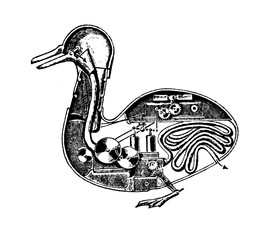
\includegraphics[scale=0.8]{imagenes/digestingduck.jpg}
	\caption{Año 1738. Autómata con forma de pato de Jacques de Vaucanson.} \label{fig:duck}
\end{figure}

\noindent Con la Revolución Industrial y el desarrollo de la tecnología comenzaron a crearse robots más complejos con motores y energía eléctrica, con formas humanoides. En el año 1917, Karel Čapek publicó Rossum's Universal Robots, que dio lugar al término \textit{robot}; además, Isaac Asimov, escribió un libro, ``Runaround'' (``Círculo vicioso''), en 1942, en el que aparecía por primera vez la palabra \textit{robótica} y se establecían las leyes de los robots. \\

\noindent Joe Engleberger junto con George Devol, lanzaron al mercado el primer robot que se comercializaría (\ref{fig:unim}), con lo que Joe Engleberger comenzó a ser considerado el padre de la robótica, ya que creó la primera empresa dedicada a este campo, \textit{Unimation} con robots preparados para la industria en los años 1950 y 1960. \\

\begin{figure}[!h]
	\centering % si queremos la imagen centrada
	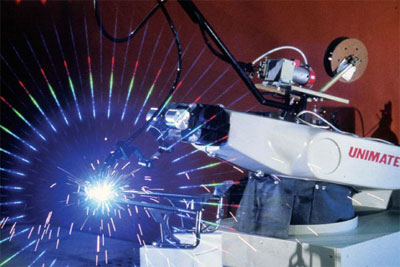
\includegraphics[scale=0.5]{imagenes/unimate.jpg}
	\caption{Año 1956. Robot industrial Unimate.} \label{fig:unim}
\end{figure}

\noindent Siguieron construyéndose robots utilizados en distintas ramas, como la industria, el espacio o destinados a la interacción con el ser humano. \\
\noindent Entre algunos impulsores de la robótica, se encuentra Rodney Brooks \cite{rodneybrooks}, el director y presidente de Rethink Robotics; fue un estudiante de matemáticas que recibió un Ph.D. en informática y que más tarde ejerció de profesor de robótica. Fundó el laboratorio de Ciencias de la Computación e Inteligencia Artificial y cofundó iRobot. En 2008 fundó la empresa Rethink Robotics.

\subsubsection{Actualidad}
\label{actualidad}
\noindent La evolución del desarrollo de robots ha permitido que estos trabajen en muchas áreas, como la industria, permitiendo una más rápida adaptación al cambio, así como un trabajo más preciso y con menos errores. Es frecuente a día de hoy decir que los robots generan desempleo, sin embargo, no existen para sustituir a una persona, sino para realizar aquellos trabajos en los que la repetición de procesos y la necesaria cualidad de que se hagan de forma rápida abundan. Cabe decir que muchos de estos trabajos suelen ser incluso peligrosos para las personas \cite{tadele2014safety}, ya que es probable que con la reiteración que supone el realizar estas tareas, el humano se equivoque, cuando un robot no lo hace \cite{brown1994human}. \\
\noindent Puesto que la robótica está obteniendo una gran presencia en la actualidad, es necesario que la sociedad se adapte a este nuevo paradigma, generando nueva formación y empleo de más valor añadido, como por ejemplo ingenieros industriales, ingenieros de automatización, programadores, etc. Además, conforme este proceso se haga más complejo, se hará necesaria la supervisión continuada por parte de especialistas, técnicos, etc. \\

\begin{figure}[H]
	\centering % si queremos la imagen centrada
	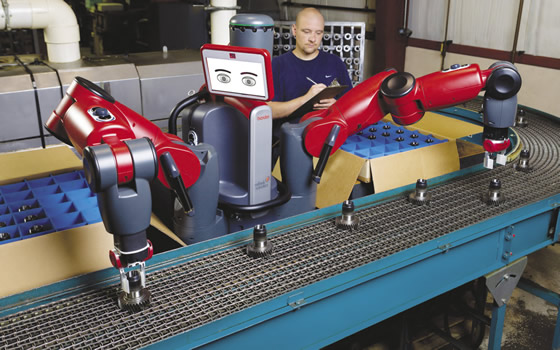
\includegraphics[scale=0.4]{imagenes/bpersona.jpeg}
	\caption{Baxter trabajando cerca de una persona.}
\end{figure}

\noindent En cuanto a Baxter, es un robot con dos brazos robóticos que, a parte de ser un robot seguro \cite{reardon2015towards} y que puede trabajar con personas como se verá en próximas secciones, no es tan caro. Según RobotWorx \cite{robots}, una compañía centrada en robótica de alta calidad a bajo precio, un robot industrial nuevo consistente en un sólo brazo robótico puede llegar a costar entre 50000 y 80000 dólares, sin incluir periféricos de aplicación específicos, con los que el precio puede aumentar hasta los 150000 dólares. En cambio, Baxter cuesta 35000 dólares incluyendo un año de garantía y un año de actualizaciones software, además de las pinzas y la bomba de vacío. \\

\noindent Estos robots industriales en principio tienen este precio, pero después es necesario añadir el coste de las infraestructuras que los rodeen para mantener a los humanos seguros. Generalmente son más difíciles de programar mientras que Baxter no requiere tanta experiencia y puede programarse para realizar varias tareas rápidamente. 




\newpage
\newpage
\section{Entorno operacional}

\noindent En este apartado se explicará el software utilizado así como el robot Baxter y sus componentes. Se comenzará con ROS, el middleware que permite integrar las tareas de control, y a continuación se hablará de MoveIt! y RViz y las plataformas utilizadas para realizar la manipulación y visualización del modelo y del movimiento. \\

\subsection{ROS}

\noindent Robotic Operating System \cite{ROS} \cite{ROS2} es un framework libre orientado a desarrollo de aplicaciones para robots. Actúa como un sistema operativo incluyendo abstracción de hardware, transferencia de mensajes entre procesos, administración de paquetes, etc. Para el desarrollo de software cuenta con librerías y herramientas que permiten construir, ejecutar y escribir código en cualquier lenguaje de programación. \\
\noindent Cada versión de ROS está montada sobre un sistema basado en Unix, aunque actualmente se está integrando en otros sistemas como Windows. \\


\subsubsection{Conceptos}
\noindent En ROS existen una serie de conceptos básicos a integrar:

\begin{itemize}
	\item Paquetes. Son la unidad básica de organización de ROS y contienen los nodos, librerías y ficheros de configuración como CMakeLists.txt y package.xml. Se pueden construir a partir de la orden catkin\_create\_package, que crea automáticamente los archivos de configuración.
	\item Nodos. Son los procesos de ROS, que pueden actuar como \textit{publishers} o \textit{subscribers} para enviar o recibir datos entre ellos.
	\item Mensajes. Son las estructuras de datos con las que se comunican los nodos.
	\item Tópicos. Son la vía de transporte de los mensajes, donde estos se publican.
	\item Servicios. Son otra forma de comunicación de los nodos vía petición/respuesta. 
	\item Comandos. Son una serie de órdenes para navegar por el sistema de ficheros y modificar o mostrar tópicos y mensajes. \\
\end{itemize}


\subsection{Baxter}

\begin{figure}[H]
	\centering % si queremos la imagen centrada
	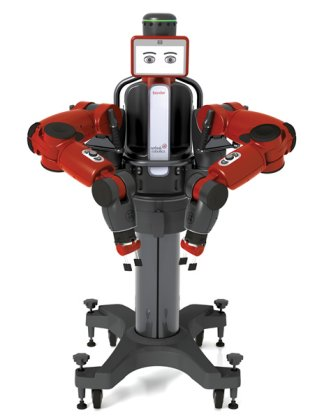
\includegraphics[scale=0.5]{imagenes/baxter1.jpg}
	\caption{Robot Baxter.}
\end{figure}

\subsubsection{Introducción}
\noindent Baxter \cite{Baxter} es un robot de automatización de procesos, desarrollado por Rethink Robotics y a la venta en el año 2012. Presenta siete grados de libertad en cada brazo y tres cámaras que se pueden utilizar o integrar en sus dos versiones disponibles: Baxter para fabricación, que incluye un entorno gráfico de fácil acceso al usuario que le permite ser programado de forma rápida y sencilla, y Baxter para investigación, para el que es necesario constar de una estación de trabajo con un entorno SDK de ROS. \\

\noindent Dos de las tres cámaras a color están situadas en los brazos y la tercera en la cabeza, donde además presenta un conjunto de sensores de ultrasonidos. Aunque consta de tres cámaras \cite{Baxter2}, sólo se pueden utilizar dos a la vez debido a las limitaciones de los USB en un entorno 64-bit.

\noindent Baxter es un robot seguro, cuenta con un botón de emergencia que deshabilita automáticamente la energía que le llega a sus componentes, de forma que cesa el proceso actual. Además consta de mecanismos de prevención de colisiones consigo mismo y, gracias a los sensores de ultrasonidos, con personas. \cite{Baxter3} \\


\subsubsection{Componentes hardware}
\label{chw}
\noindent Como se ha mencionado antes, cada brazo robótico \cite{Baxter4} tiene siete grados de libertad, lo que le permite realizar casi todos los movimientos que puede realizar un brazo humano, aunque este último conste de unos 26 grados de libertad. \\

\noindent Se utilizan actuadores elásticos que consisten en introducir un resorte entre el motor y los engranajes de las articulaciones de Baxter, proporcionando más seguridad, menos ruido de control y más estabilidad. \\

\noindent En cada brazo hay sensores infrarrojos, un acelerómetro, botones para navegar en la interfaz y, como se ha dicho anteriormente, cámaras. \\

\noindent Para nombrar cada una de las articulaciones se utilizan varias letras: S para los ``hombros'' (\textit{shoulder}), E para los ``codos'' (\textit{elbow}) y W para las ``muñecas'' (\textit{wrist}), con un número que indicará el ángulo de navegación \cite{AN}, un tipo de ángulo de Euler que se describe a continuación.

\begin{itemize}
	\item Dirección o \textit{yaw}. Rotación contraria a las agujas del reloj en el eje Z.
	\item Elevación o \textit{pitch}. Rotación contraria a las agujas del reloj en el eje Y.
	\item Ángulo de alabeo o \textit{roll}. Rotación contraria a las agujas del reloj en el eje X.
\end{itemize}

\noindent En la figura (\ref{fig:arm}) vemos cómo se denomina cada articulación de los brazos de Baxter.

\begin{figure}[H]
	\centering % si queremos la imagen centrada
	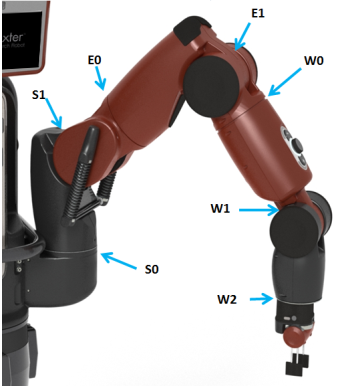
\includegraphics[scale=0.6]{imagenes/Baxter_arm.png}
	\caption{Articulaciones de Baxter.} \label{fig:arm}
\end{figure}

\noindent S0 - Shoulder Roll,
S1 - Shoulder Pitch,
E0 - Elbow Roll,
E1 - Elbow Pitch,
W0 - Wrist Roll,
W1 - Wrist Pitch,
W2 - Wrist Roll.\\

\noindent Existen dos tipos de pinzas o \textit{grippers} que se pueden colocar en los brazos de Baxter: los eléctricos y los aspiradores. Los eléctricos son dos palas paralelas que pueden levantar hasta 2 kilos aproximadamente; en cuanto a los aspiradores, se utilizan para coger objetos succionando, para lo que es necesario conectar un suministro de aire externo. \\


\subsection{MoveIt! y RViz}
\noindent MoveIt! \cite{moveit} es una plataforma de código abierto montada sobre ROS enfocada a manipulación de robots, control, cinemáticas, detección de colisiones y navegación. En este proyecto se ha utilizado para la definición de trayectorias, planificación y ejecución de las mismas, así como la detección de colisiones.\\
\noindent Para utilizar este software es necesario proporcionar el archivo URDF (es decir, el formato de modelos de robots de ROS) del robot utilizado, y MoveIt! se encarga de generar todos los archivos para comenzar a trabajar. \\
\noindent MoveIt! utiliza verificadores de colisión como FCL, una librería que detecta solapamientos entre modelos \cite{moveitfaq}. \\

\noindent El plugin RViz \cite{rviz} es una GUI de ROS (ROS Visualizer) que sirve para visualizar el modelo de robot, configurar la planificación de movimientos, evitar colisiones, además de consultar valores de los tópicos de ROS como los de las cámaras, sensores infrarrojos, etc. Normalmente se utiliza como librería de planificación la librería OMPL, de código abierto y alta calidad de planificación aleatoria. \\


\subsection{Modelos de robot}
\subsubsection{Formato universal de descripción robótica}
\noindent Este archivo URDF (\textit{Universal Robotic Description Format}), contiene la representación en formato XML del modelo de robot en estructura de árbol\cite{models2}, que, en caso de Baxter, se genera dinámicamente al iniciarlo, y actualizado cuando se conectan o desconectan los \textit{grippers} o pinzas o cuando se coge o suelta un objeto \cite{models}. Contiene información sobre la descripción cinemática o dinámica del robot, representación visual, modelo de colisión y enlaces entre las articulaciones \cite{models3} [p. 60-61]. \\


\subsubsection{Formato semántico de descripción robótica}

\noindent El archivo SRDF (\textit{Semantic Robot Description Format}) se genera dinámicamente al iniciar MoveIt! y complementa al archivo URDF. Contiene los parámetros necesarios para establecer los límites de las articulaciones de los brazos y articulaciones virtuales, información sobre cinemática y controladores y verificadores de colisión adicionales \cite{models3} [p. 122]. \\

\newpage
%
\section{Gestión del proyecto}
\label{software}
\noindent En este apartado se expone la planificación seguida en el proyecto, dividido en las tareas que lo componen, mostrando algunas dificultades, problemas y tiempo invertido en cada una de ellas, así como el presupuesto estimado del trabajo realizado.

\subsection{Metodología del software}
\noindent La metodología utilizada en este proyecto ha sido el desarrollo en espiral, en el que cada iteración representa un conjunto de actividades y la siguiente se elige en función del análisis de riesgo de las anteriores. De esta forma, este modelo itera repetidamente mejorando cualquier tipo de conflictos en la implementación, reduciéndolos conforme se completan las iteraciones \cite{boehm1988spiral}.

\subsection{Planificación}

\noindent Para organizar la planificación seguida en este proyecto, se muestra el diagrama de Gantt (figura \ref{fig:gantt}) desde el 07/03/2018 hasta el 06/06/2018: \\

\begin{figure}[H]
	\centering
	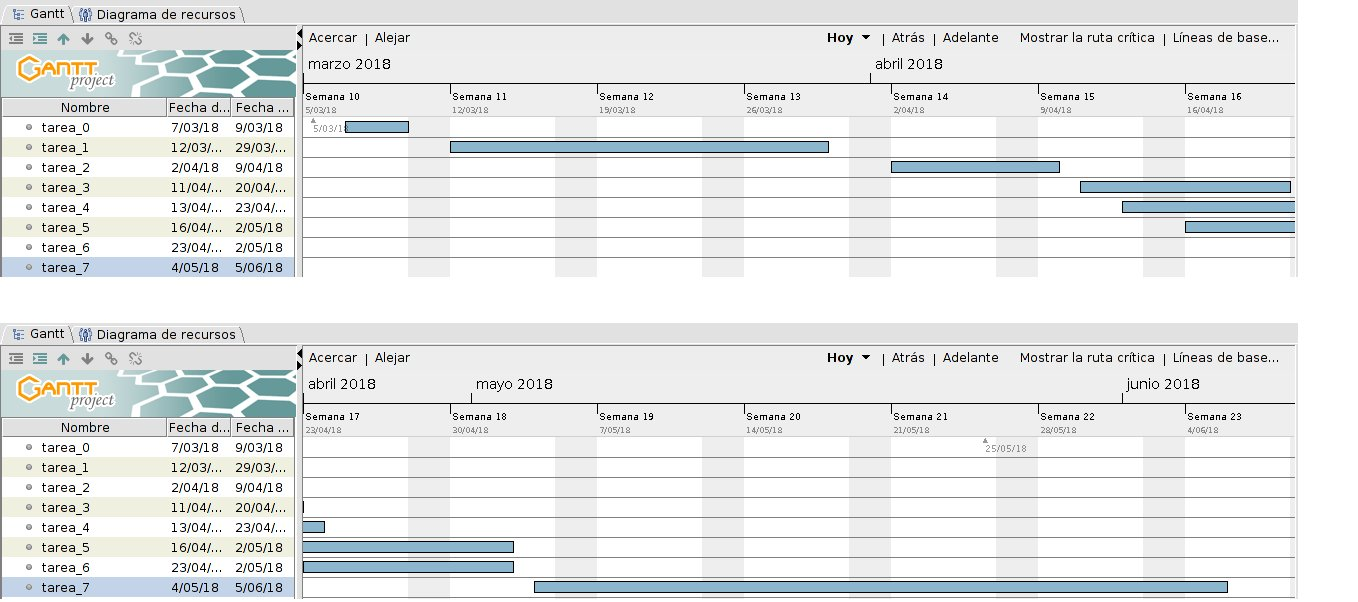
\includegraphics[width=1.5\textwidth, angle=90]{imagenes/gantt.jpg}
	\label{fig:gantt}
	\caption{Diagrama de Gantt.}
\end{figure}

\begin{table}[!h]
	\centering
	\begin{tabular}{|p{2cm} | p{5cm} | p{2cm} | p{2cm} | p{2cm} |}
		\hline
		\textbf{Tarea} & \textbf{Nombre} & \textbf{Fecha de inicio} & \textbf{Fecha de fin} & \textbf{Estimación} \\
		\hline
		tarea\_0 & Instalación y toma de conceptos de MoveIt! y ROS & 07/03/2018 & 10/03/2018 & 4 días\\
		\hline
		tarea\_1 & Adaptación de software \textit{pick and place} utilizando módulos de visión & 12/03/2018 & 30/03/2018 & 18 días \\
		\hline
		tarea\_2 & Estudio de visión por computador & 02/04/2018 & 10/04/2018 & 8 días \\
		\hline
		tarea\_3 & Estudio de algoritmo k-medias e implementación en C++ & 11/04/2018 & 21/04/2018 & 10 días \\
		\hline 
		tarea\_4 & Desarrollo de software de visión por computador & 13/04/2018 & 23/04/2018 & 10 días \\
		\hline
		tarea\_5 & Desarrollo de software de clasificación en entorno estático & 16/04/2018 & 03/04/2018 & 17 días \\
		\hline
		tarea\_6 & Desarrollo de software de clasificación en entorno dinámico & 23/04/2018 & 03/05/2018 & 11 días \\
		\hline
		tarea\_7 & Realización de pruebas y corrección de errores & 04/05/2018 & 06/06/2018 & 30 días \\
		\hline
		
	\end{tabular}
	\caption{Planificación de proyecto.}
	\label{cuad:plan}
\end{table}

\newpage
\subsection{Presupuesto}

\subsubsection{Recursos hardware y software}

\noindent Para hacer el presupuesto de este proyecto se ha utilizado la fórmula siguiente:
\begin{center}
	$ (D/V) * C $
\end{center}

\noindent Donde:
\begin{itemize}
	\item D es el número de meses que se ha utilizado el producto para el proyecto.
	\item V es la vida útil del producto en número de meses.
	\item C es el coste total del producto en euros. \\
\end{itemize}

\begin{table}[H]
	\centering
	\begin{tabular}{|p{2cm} | p{2cm} | p{2cm} | p{2cm} | p{2cm} |}
		\hline % para poner una linea horizontal
		\textbf{Artículo} & \textbf{Coste} (euros) & \textbf{Dedicación} (meses) & \textbf{Vida Útil} (meses) & \textbf{Coste Aplicable} (euros)\\ % el & se usa para separar columnas y el \\ para saltos de linea
		\hline	
		Baxter & 24078\euro & 4 & 120 & 802,6\euro \\
		\hline
		Ordenador de sobremesa & 1500\euro & 4 & 60 & 100\euro \\
		\hline
		Cinta transportadora & 350\euro & 2 & 120 & 5,83\euro \\
		\hline
		Total & \multicolumn{4}{r|}{868,43\euro} \\ 
		\hline
	\end{tabular}
	\caption{Tabla de costes.}
\end{table}

\subsubsection{Recursos humanos}
\noindent En este trabajo se han empleado aproximadamente 80 días, contando con que una jornada laboral común suelen ser 8 horas al día y con que además de este proyecto se ha trabajado en otras asignaturas, se considera que en media se han invertido 4 horas al día. \\

\noindent Suponiendo que un ingeniero informático recién graduado en España representa un coste de 2000 euros al mes, las 320 horas del proyecto estarían valoradas en 1731.2 euros en total. \\


\subsubsection{Coste total}
\begin{table}[H]
	\centering
	\begin{tabular}{|p{4cm} | p{4cm} |}
		\hline
		\multicolumn{2}{|c|}{\textbf{COSTE TOTAL}} \\
		\hline 
		Recursos HW y SW & 868\euro \\
		\hline
		Recursos humanos & 1731\euro \\
		\hline
		Coste total & 2599\euro \\
		\hline
	\end{tabular}
	\caption{Coste total del proyecto}
	\label{cuad:ct}
\end{table}

\noindent Por lo tanto, añadiendo un 20\% referido a gastos, el coste total del proyecto sería de: \\

PRECIO TOTAL: 3120\euro (IVA no incluido)\\

\subsection{Gestión de problemas}
\label{planif}
\noindent En este proyecto se han enfrentado muchos problemas de los que se hablará en este apartado. Se hacía imprescindible su resolución, ya que suponían un impacto grave en el funcionamiento del código.\\

\noindent \textbf{Problema 1. Incompatibilidades a la hora de utilizar las plataformas MoveIt!, Gazebo y ROS sobre Ubuntu 16.04 LTS en el portátil personal.} No se propuso ninguna solución, puesto que en el laboratorio había un servidor disponible con Ubuntu 14.04.5 LTS y ROS Indigo. \\

\noindent \textbf{Problema 2. Actualización en el servidor del laboratorio.} Debido a una actualización de Windows, la gráfica de este computador quedó inutilizable. Para resolver este problema, se formateó el servidor, instalando ROS Kinetic sobre Ubuntu 16.04 LTS y MoveIt! (esta vez no resultó necesario instalar el simulador Gazebo, ya que este servidor se encuentra en el mismo lugar que el robot Baxter). \\

\noindent \textbf{Problema 3. Planificación de MoveIt!.} A la hora de utilizar OMPL, el algoritmo de planificación de MoveIt!, el resultado obtenido no siempre es el esperado; en ocasiones, al intentar ejecutar movimientos simples, el algoritmo recalcula la posición de las articulaciones de Baxter de forma que esta sea la óptima, sin embargo, resulta en un movimiento del brazo robótico más espaciado que impide realizar la clasificación correctamente. Para solucionarlo se implementan como movimientos pequeñas variaciones con respecto a la posición que el brazo tenía anteriormente.\\

%\noindent A la hora de la separación, cuando el \textit{gripper} de Baxter ya se encontraba en el punto medio, surgía otro problema al rotar el \textit{gripper} hacia la posición horizontal, ya que este giraba en el mismo sentido en todas las ocasiones. Esto no siempre era un problema, ya que algunas ejecuciones dejaban el brazo en el mejor caso posible, pero resultaba muy ineficiente en los casos en los que no era así. \\
%\noindent Esto podía resolverse comprobando si la orientación superaba $\pi$/4, en ese caso cambiabamos el sentido de la orientación.\\

%\noindent Baxter muy lento

\noindent \textbf{Problema 4. Permisos de ejecución.} ROS suele expresar los errores como \textit{``Process is dead''}. Normalmente especifica anteriormente el porqué, pero en este caso no lo hacía. El problema era que el programa escrito en Python no tenía permisos de ejecución. \\


\noindent \textbf{Problema 5. Iluminación.} La iluminación es una característica clave en un programa que utiliza visión por computador, y son muchos los problemas que esta puede dar, un ejemplo son los focos, ya que aunque no los veamos, están parpadeando constantemente, esto influye al capturar las imágenes de los objetos. Existen focos de luz azul capaces de solucionar esto; en mi caso, utilicé la luz natural y alguna artificial de la sala, intentando crear sombras para que esta no incidiese directamente sobre los objetos.\\

\noindent \textbf{Problema 6. Entrada del algoritmo K-means.} El problema principal consistía en que el único tipo de dato que se le puede pasar a este algoritmo es \textit{Mat} de OpenCV. Puesto que se estaba trabajando con \textit{PoseArray} de ROS para obtener las coordenadas en la imagen, se intentó adaptar para pasárselo a K-means. Este consiste en un array de \textit{PoseStamped}, un tipo de dato que incluye unas coordenadas para especificar la posición del objeto y otras para la orientación. Puesto que el objetivo más básico del proyecto era realizar una segmentación por color y posición y al algoritmo no se le podían pasar valores RGB ya que la salida resultaría ser otro valor intermedio RGB y no una posición entre los dos clústers, se definió específicamente un valor para cada objeto que indicaba su color y se mandaba a través de la coordenada \textit{z}, ya que no es necesario especificarla porque los objetos siempre se mantienen en la misma \textit{z} (sobre la mesa o cinta transportadora). Así, la posición, orientación y color del objeto se incluyen en la matriz \textit{Mat} para obtener los dos clústers tras ejecutar K-means.\\
%
\newpage
\newpage
\section{Análisis y diseño del sistema}
\noindent En esta sección se especificarán los casos de uso que componen el sistema, además de los requisitos funcionales y no funcionales para ambas clasificaciones, estática y dinámica, en este último caso utilizando una cuña como herramienta de separación. \\

\noindent Las principales características funcionales son:
\begin{itemize}
	\item Mover los brazos de Baxter a la posición inicial (figura \ref{cd:ip}) con la que comenzará todas sus ejecuciones.
	\begin{figure}[!h]
		\label{cd:ip}
		\centering % si queremos la imagen centrada
		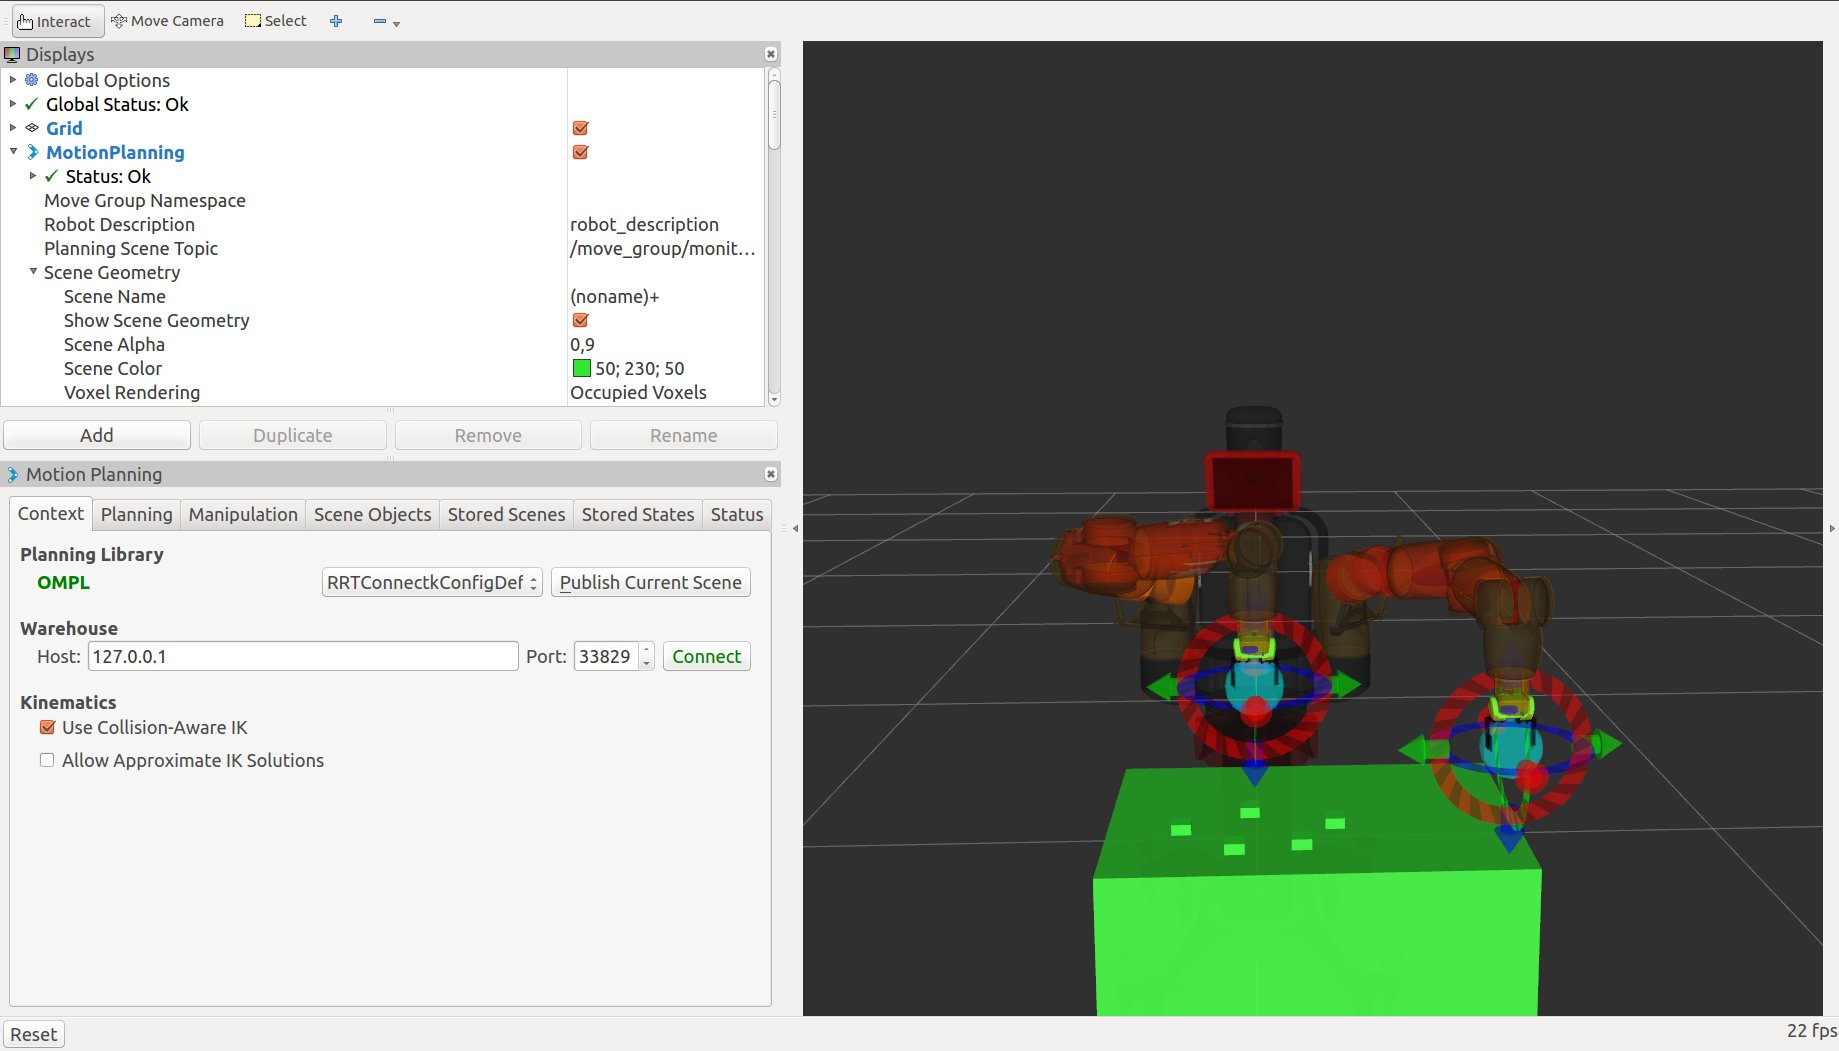
\includegraphics[scale=0.22]{imagenes/initialpos.jpg}
		\caption{Posición inicial de Baxter.}
	\end{figure}
	\item Visión por computador para obtener la imagen de los objetos sobre la mesa o cinta transportadora.
	\item Reconocimiento de objetos.
	\item Si no se reconoce ningún objeto, Baxter no hará nada hasta que sean identificados.
	\item Obtención de información acerca de la posición de los objetos a través de los tópicos de ROS.
	\item Si se trata de clasificación en entorno estático, se procederá a situar el brazo de Baxter entre los objetos con la orientación adecuada para separarlos.
	\item Si, por contrario, se trata de clasificación en entorno dinámico, Baxter llevará la cuña a un punto cercano al punto medio, y conforme los objetos vayan llegando al punto medio obtenido, moverá la cuña con la orientación necesaria para separarlos.
\end{itemize}

\subsection{Restricciones del sistema}

\subsubsection{Restricciones hardware}

\begin{itemize}
	\item El rango de movimiento del brazo derecho (el brazo utilizado) de Baxter es limitado. A la hora de calcular la posición en la que pueden estar los objetos tras un determinado tiempo es posible obtener una posición a la que Baxter no pueda llegar.
	\item No se puede controlar la planificación OMPL realizada por MoveIt!, por lo que no se puede conocer a ciencia cierta cómo va a realizar el movimiento o cuánto va a tardar en realizarlo, siendo la velocidad máxima 1m/s.
	\item Baxter tiene que estar conectado a la corriente.
	\item La cinta transportadora utilizada es estrecha, por lo que no caben muchos objetos.
	\item La cinta transportadora consta de 10 velocidades que se controlan mediante una rueda. 
	\item Es importante disponer de una iluminación suficiente como para que el sistema de reconocimiento identifique los objetos, evitando la aparición de reflejos y artefactos. \\
\end{itemize}

\subsubsection{Restricciones software}
\begin{itemize}
	\item Es necesario realizar este proyecto sobre un directorio RSDK (conexión entre el PC y el robot mediante ROS) de ROS.
	\item En este caso se ha utilizado ROS Kinetic, por lo que sólo se ha podido montar sobre Ubuntu 16.04 LTS, Xenial.
	\item El lenguaje de programación utilizado para la parte de visión por computador será C++, y para el control, Python. \\
\end{itemize}

\subsection{Especificación de casos de uso}
\noindent Los casos de uso describen cómo interactúa un actor con el entorno.\cite{cu} \\
\noindent Las tareas de este proyecto son realizadas por Baxter y el programa de visión por computador.
\begin{itemize}
	\item \textbf{Software de reconocimiento.} Este programa se encarga de procesar la información que llega de las cámaras de Baxter y enviarla ya procesada de nuevo al robot.
	\item \textbf{Baxter.} Se encarga de realizar los movimientos correspondientes utilizando la información que le llega del software de visión. \\
\end{itemize}

\noindent A continuación se muestra el diagrama de casos de uso a seguir para describir cada uno de ellos. \\

\begin{figure}[!h]
	\label{cd:cud}
	 % si queremos la imagen centrada
	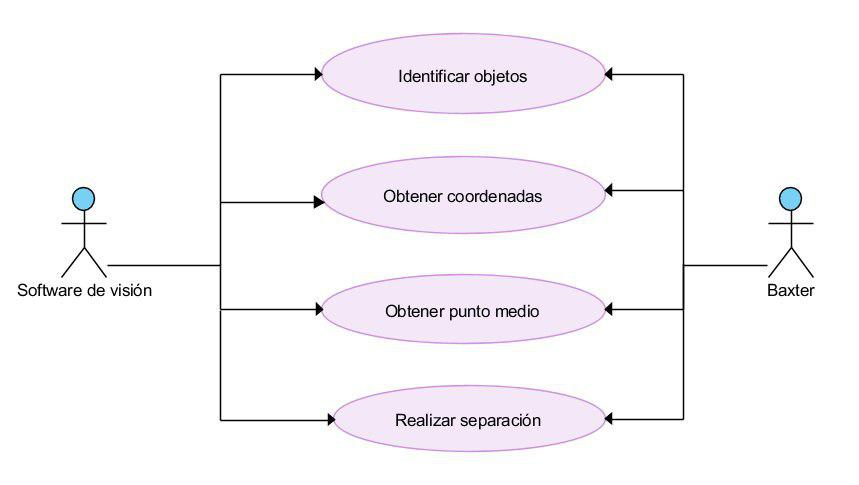
\includegraphics[scale=0.6]{imagenes/cud.jpg}
	\caption{Diagrama de casos de uso.}
\end{figure}

\begin{table}[H]
	\centering
	\begin{tabular}{|p{2.5cm} | p{6cm} | p{5cm} |}
		\hline
		\textbf{Caso de Uso} & Reconocimiento de objetos & \textbf{CU-001} \\
		\hline 
		Actor & \multicolumn{2}{|l|}{Baxter y software de visión} \\
		\hline
		Tipo & \multicolumn{2}{|l|}{Principal | Real} \\
		\hline
		Referencias & RF-001 \ref{cuad:RF-001}, RF-002 \ref{cuad:RF-002}, RF-003 \ref{cuad:RF-003}, RF-004 \ref{cuad:RF-004}, RF-007 \ref{cuad:RF-007}, RNF-001 \ref{cuad:RNF-001}, RNF-002 \ref{cuad:RNF-002} & CU-004 \ref{cuad:CU-002}, CU-003 \ref{cuad:CU-003}, CU-004 \ref{cuad:CU-004}, CU-005 \ref{cuad:CU-005}, CU-006 \ref{cuad:CU-006}, CU-007 \ref{cuad:CU-007}, CU-008 \ref{cuad:CU-007}, CU-008 \ref{cuad:CU-008}, CU-009 \ref{cuad:CU-009} \\
		\hline
		Precondiciones & \multicolumn{2}{|l|}{\parbox{30em}{Los objetos deben estar en el rango de visión de la cámara de Baxter y la iluminación debe permitir reconocerlos.}} \\
		\hline
		Poscondiciones & \multicolumn{2}{|l|}{Se conocerá el centro de los objetos reconocidos en la imagen.}\\
		\hline
		Propósito & \multicolumn{2}{|l|}{\parbox{30em}{Conocer los objetos que hay sobre la mesa o cinta transportadora para clasificarlos.}} \\
		\hline
		Resumen & \multicolumn{2}{|l|}{\parbox{30em}{El software de visión se encarga de reconocer y obtener el punto medio de los objetos que le llegan de la cámara de Baxter.}} \\
		\hline
		
	\end{tabular}
	\caption{Caso de uso CU-001.}
	\label{cuad:CU-001}
\end{table}

\begin{table}[H]
	\centering
	\begin{tabular}{|p{2.5cm} | p{6cm} | p{5cm} |}
		\hline
		\textbf{Caso de Uso} & Obtención del punto medio & \textbf{CU-002} \\
		\hline 
		Actor & \multicolumn{2}{|l|}{Software de visión} \\
		\hline
		Tipo & \multicolumn{2}{|l|}{Secundario | Real} \\
		\hline
		Referencias & RF-003 \ref{cuad:RF-003}, RF-004 \ref{cuad:RF-004}, RF-005 \ref{cuad:RF-005}, RF-007 \ref{cuad:RF-007}, RNF-001 \ref{cuad:RNF-001}, RNF-002 \ref{cuad:RNF-002} & CU-001 \ref{cuad:CU-001}, CU-003 \ref{cuad:CU-003}, CU-004 \ref{cuad:CU-004}, CU-005 \ref{cuad:CU-005}, CU-006 \ref{cuad:CU-006}, CU-007 \ref{cuad:CU-007}, CU-008 \ref{cuad:CU-007}, CU-008 \ref{cuad:CU-008}, CU-009 \ref{cuad:CU-009} \\
		\hline
		Precondiciones & \multicolumn{2}{|l|}{\parbox{30em}{Se deben haber reconocido objetos en la mesa. El algoritmo k-medias debe haberse ejecutado correctamente.}} \\
		\hline
		Poscondiciones & \multicolumn{2}{|l|}{Se conocerá el punto medio de los dos clústers.}\\
		\hline
		Propósito & \multicolumn{2}{|l|}{Conocer el punto medio para situar en él el brazo robótico.} \\
		\hline
		Resumen & \multicolumn{2}{|l|}{\parbox{30em}{El software de visión obtiene a partir del algoritmo k-medias la posición de dos clústers de los que calcula el punto medio.}} \\
		\hline
		
	\end{tabular}
	\caption{Caso de uso CU-002.}
	\label{cuad:CU-002}
\end{table}

\subsubsection{Entorno estático}

\noindent Además de los casos de uso \ref{cuad:CU-001} y \ref{cuad:CU-002}, para realizar la clasificación en entorno estático es necesario el siguiente paso. \\

\begin{table}[H]
	\centering
	\begin{tabular}{|p{2.5cm} | p{6cm} | p{5cm} |}
		\hline
		\textbf{Caso de Uso} & Situar brazo en punto medio en entorno estático & \textbf{CU-003} \\
		\hline 
		Actor & \multicolumn{2}{|l|}{Baxter} \\
		\hline
		Tipo & \multicolumn{2}{|l|}{Primario | Esencial} \\
		\hline
		Referencias & RF-005 \ref{cuad:RF-005}, RF-006 \ref{cuad:RF-006}, RF-007 \ref{cuad:RF-007}, RNF-001 \ref{cuad:RNF-001}, RNF-002 \ref{cuad:RNF-002} & CU-001 \ref{cuad:CU-001}, CU-002 \ref{cuad:CU-002}, CU-004 \ref{cuad:CU-004}, CU-005 \ref{cuad:CU-005} \\
		\hline
		Precondiciones & \multicolumn{2}{|l|}{\parbox{30em}{Haber obtenido el punto medio entre los dos clústers con el algoritmo k-medias.}} \\
		\hline
		Poscondiciones & \multicolumn{2}{|l|}{\parbox{30em}{El brazo robótico se situará en el punto medio entre los clústers con una orientación perpendicular a la que forma la recta que une los dos clústers.}}\\
		\hline
		Propósito & \multicolumn{2}{|l|}{\parbox{30em}{Situar el brazo de Baxter en el punto medio con la orientación necesaria para realizar la clasificación.}} \\
		\hline
		Resumen & \multicolumn{2}{|l|}{\parbox{30em}{Baxter mueve su brazo derecho al punto medio a partir de los datos obtenidos mediante tópicos de ROS.}} \\
		\hline
		
	\end{tabular}
	\caption{Caso de uso CU-003.}
	\label{cuad:CU-003}
\end{table}

\begin{table}[H]
	\centering
	\begin{tabular}{|p{2.5cm} | p{6cm} | p{5cm} |}
		\hline
		\textbf{Caso de Uso} & Rotar paleta en entorno estático & \textbf{CU-004} \\
		\hline 
		Actor & \multicolumn{2}{|l|}{Baxter} \\
		\hline
		Tipo & \multicolumn{2}{|l|}{Primario | Esencial} \\
		\hline
		Referencias & RF-005 \ref{cuad:RF-005}, RF-006 \ref{cuad:RF-006}, RF-007 \ref{cuad:RF-007}, RNF-001 \ref{cuad:RNF-001}, RNF-002 \ref{cuad:RNF-002} & CU-001 \ref{cuad:CU-001}, CU-002 \ref{cuad:CU-002}, CU-003 \ref{cuad:CU-003}, CU-005 \ref{cuad:CU-005} \\
		\hline
		Precondiciones & \multicolumn{2}{|l|}{\parbox{30em}{Haber obtenido el punto medio entre los dos clústers y haber situado en él el gripper con la orientación calculada.}} \\
		\hline
		Poscondiciones & \multicolumn{2}{|l|}{\parbox{30em}{El gripper girará hasta que se encuentre paralelo al eje horizontal.}}\\
		\hline
		Propósito & \multicolumn{2}{|l|}{\parbox{30em}{Rotar el gripper de forma que se pueda realizar más fácilmente la separación.}} \\
		\hline
		Resumen & \multicolumn{2}{|l|}{\parbox{30em}{Se rota el gripper de Baxter de forma que los objetos quedan separados por una recta horizontal.}} \\
		\hline
		
	\end{tabular}
	\caption{Caso de uso CU-004.}
	\label{cuad:CU-004}
\end{table}

\begin{table}[H]
	\centering
	\begin{tabular}{|p{2.5cm} | p{6cm} | p{5cm} |}
		\hline
		\textbf{Caso de Uso} & Separar objetos en entorno estático & \textbf{CU-005} \\
		\hline 
		Actor & \multicolumn{2}{|l|}{Baxter} \\
		\hline
		Tipo & \multicolumn{2}{|l|}{Primario | Esencial} \\
		\hline
		Referencias & RF-005 \ref{cuad:RF-005}, RF-006 \ref{cuad:RF-006}, RF-007 \ref{cuad:RF-007}, RNF-001 \ref{cuad:RNF-001}, RNF-002 \ref{cuad:RNF-002} & CU-001 \ref{cuad:CU-001}, CU-002 \ref{cuad:CU-002}, CU-003 \ref{cuad:CU-003}, CU-004 \ref{cuad:CU-004} \\
		\hline
		Precondiciones & \multicolumn{2}{|l|}{\parbox{30em}{Tener situado el gripper en el punto medio con una orientación paralela al eje horizontal.}} \\
		\hline
		Poscondiciones & \multicolumn{2}{|l|}{\parbox{30em}{El brazo se desplazará en el eje vertical para separar los objetos.}}\\
		\hline
		Propósito & \multicolumn{2}{|l|}{\parbox{30em}{Separar los objetos mediante movimientos en el eje vertical de Baxter.}} \\
		\hline
		Resumen & \multicolumn{2}{|l|}{\parbox{30em}{Desplazar el brazo arriba y abajo en el eje vertical separando los objetos conforme a color y posición.}} \\
		\hline
		
	\end{tabular}
	\caption{Caso de uso CU-005.}
	\label{cuad:CU-005}
\end{table}

\subsubsection{Entorno dinámico}
\noindent Para realizar la clasificación con una cuña como herramienta y una cinta transportadora sobre la que se sitúan los objetos, además del caso de uso \ref{cuad:CU-001}, es necesario lo siguiente. \\

\begin{table}[H]
	\centering
	\begin{tabular}{|p{2.5cm} | p{6cm} | p{5cm} |}
		\hline
		\textbf{Caso de Uso} & Cálculo de la velocidad en entorno dinámico & \textbf{CU-006} \\
		\hline 
		Actor & \multicolumn{2}{|l|}{Software} \\
		\hline
		Tipo & \multicolumn{2}{|l|}{Secundario | Real} \\
		\hline
		Referencias & RF-004 \ref{cuad:RF-004}, RF-005 \ref{cuad:RF-005}, RF-006 \ref{cuad:RF-006}, RF-007 \ref{cuad:RF-007}, RNF-001 \ref{cuad:RNF-001}, RNF-002 \ref{cuad:RNF-002} & CU-001 \ref{cuad:CU-001}, CU-002 \ref{cuad:CU-002}, CU-007 \ref{cuad:CU-007}, CU-008 \ref{cuad:CU-008}, CU-009 \ref{cuad:CU-009} \\
		\hline
		Precondiciones & \multicolumn{2}{|l|}{\parbox{30em}{Haber obtenido el punto medio entre los dos clústers en dos ocasiones.}} \\
		\hline
		Poscondiciones & \multicolumn{2}{|l|}{\parbox{30em}{Se conocerá la velocidad media a la que van los objetos sobre la cinta transportadora.}}\\
		\hline
		Propósito & \multicolumn{2}{|l|}{\parbox{30em}{Obtener la velocidad a la que van los objetos para realizar la separación.}} \\
		\hline
		Resumen & \multicolumn{2}{|l|}{\parbox{30em}{Se obtiene la posición del punto medio entre los dos clústers en dos ocasiones, una al principio y otra un tiempo después y se calcula la velocidad que llevan los objetos.}} \\
		\hline
		
	\end{tabular}
	\caption{Caso de uso CU-006.}
	\label{cuad:CU-006}
\end{table}

\begin{table}[H]
	\centering
	\begin{tabular}{|p{2.5cm} | p{6cm} | p{5cm} |}
		\hline
		\textbf{Caso de Uso} & Situar brazo en posición cercana al punto medio en entorno dinámico & \textbf{CU-007} \\
		\hline 
		Actor & \multicolumn{2}{|l|}{Baxter} \\
		\hline
		Tipo & \multicolumn{2}{|l|}{Primario | Esencial} \\
		\hline
		Referencias & RF-005 \ref{cuad:RF-005}, RF-006 \ref{cuad:RF-006}, RF-007 \ref{cuad:RF-007}, RNF-001 \ref{cuad:RNF-001}, RNF-002 \ref{cuad:RNF-002} & CU-001 \ref{cuad:CU-001}, CU-002 \ref{cuad:CU-002}, CU-006 \ref{cuad:CU-006}, CU-008 \ref{cuad:CU-008}, CU-009 \ref{cuad:CU-009} \\
		\hline
		Precondiciones & \multicolumn{2}{|l|}{\parbox{30em}{Haber obtenido el último valor de punto medio entre los dos clústers y la velocidad a la que van los objetos.}} \\
		\hline
		Poscondiciones & \multicolumn{2}{|l|}{\parbox{30em}{El brazo robótico se situará en un punto cercano al punto medio aumentando la rotación del gripper.}} \\
		\hline
		Propósito & \multicolumn{2}{|l|}{\parbox{30em}{Mover el brazo a un punto cercano al punto medio para realizar el barrido necesario para clasificar los objetos.}} \\
		\hline
		Resumen & \multicolumn{2}{|l|}{\parbox{30em}{Baxter mueve su brazo derecho al punto calculado con un valor de orientación más alto que el calculado para el punto medio.}} \\
		\hline
		
	\end{tabular}
	\caption{Caso de uso CU-007.}
	\label{cuad:CU-007}
\end{table}

\begin{table}[H]
	\centering
	\begin{tabular}{|p{2.5cm} | p{6cm} | p{5cm} |}
		\hline
		\textbf{Caso de Uso} & Situar brazo en punto medio en entorno dinámico & \textbf{CU-008} \\
		\hline 
		Actor & \multicolumn{2}{|l|}{Baxter} \\
		\hline
		Tipo & \multicolumn{2}{|l|}{Primario | Esencial} \\
		\hline
		Referencias & RF-005 \ref{cuad:RF-005}, RF-006 \ref{cuad:RF-006}, RF-007 \ref{cuad:RF-007}, RNF-001 \ref{cuad:RNF-001}, RNF-002 \ref{cuad:RNF-002} & CU-001 \ref{cuad:CU-001}, CU-002 \ref{cuad:CU-002}, CU-006 \ref{cuad:CU-006}, CU-007 \ref{cuad:CU-007}, CU-009 \ref{cuad:CU-009} \\
		\hline
		Precondiciones & \multicolumn{2}{|l|}{\parbox{30em}{El gripper debe estar situado en un punto cercano al punto medio.}} \\
		\hline
		Poscondiciones & \multicolumn{2}{|l|}{\parbox{30em}{Baxter mueve el brazo hacia el último punto medio obtenido con la orientación necesaria para realizar la separación.}} \\
		\hline
		Propósito & \multicolumn{2}{|l|}{\parbox{30em}{Mover el brazo al punto medio para realizar la separación.}} \\
		\hline
		Resumen & \multicolumn{2}{|l|}{\parbox{30em}{Baxter mueve su brazo derecho al punto medio con la orientación adecuada para que los objetos queden separados.}} \\
		\hline
		
	\end{tabular}
\caption{Caso de uso CU-008}
\label{cuad:CU-008}
\end{table}

\begin{table}[H]
	\centering
	\begin{tabular}{|p{2.5cm} | p{6cm} | p{5cm} |}
		\hline
		\textbf{Caso de Uso} & Sacudida de objetos en entorno dinámico & \textbf{CU-009} \\
		\hline 
		Actor & \multicolumn{2}{|l|}{Baxter} \\
		\hline
		Tipo & \multicolumn{2}{|l|}{Primario | Esencial} \\
		\hline
		Referencias & RF-005 \ref{cuad:RF-005}, RF-006 \ref{cuad:RF-006}, RF-007 \ref{cuad:RF-007}, RNF-001 \ref{cuad:RNF-001}, RNF-002 \ref{cuad:RNF-002} & CU-001 \ref{cuad:CU-001}, CU-002 \ref{cuad:CU-002}, CU-006 \ref{cuad:CU-006}, CU-007 \ref{cuad:CU-007}, CU-008 \ref{cuad:CU-008} \\
		\hline
		Precondiciones & \multicolumn{2}{|l|}{\parbox{30em}{El brazo se encuentra en el punto medio en el que separa los objetos.}} \\
		\hline
		Poscondiciones & \multicolumn{2}{|l|}{\parbox{30em}{Baxter moverá el brazo con la misma orientación que tenía en el eje vertical para separar los objetos más satisfactoriamente.}} \\
		\hline
		Propósito & \multicolumn{2}{|l|}{\parbox{30em}{Realizar movimientos verticales con la posición actual del gripper para separar más rápido los objetos.}} \\
		\hline
		Resumen & \multicolumn{2}{|l|}{\parbox{30em}{Se mueve el brazo derecho en su posición actual en el eje vertical separando más rápidamente los objetos.}} \\
		\hline
		
	\end{tabular}
	\caption{Caso de uso CU-009.}
	\label{cuad:CU-009}
\end{table}

\subsection{Especificación de requisitos}
\noindent Los requisitos pueden ser clasificados en funcionales o no funcionales. Los funcionales se refieren a cualquier comportamiento que esté directamente relacionado con el funcionamiento del sistema, mientras que los requisitos no funcionales especifican cómo debe comportarse el sistema. \\

\subsubsection{Requisitos funcionales}
\begin{table}[H]
	\centering
	\begin{tabular}{|p{2cm} | p{1.5cm} | p{2cm} | p{1.7cm} | p{2cm} | p{2cm} |}
		\hline
		\multicolumn{6}{|c|}{\textbf{REQUISITO DEL SISTEMA}} \\ 
		\hline
		\textbf{ID} & RF-001 & & \textbf{Fuente} & \multicolumn{2}{c|}{CU-001} \\
		\hline
		\textbf{Nombre} & \multicolumn{5}{l|}{Reconocimiento de objetos} \\
		\hline
		\textbf{Descripción} & \multicolumn{5}{l|}{\parbox{30em}{Se obtienen imágenes de los objetos situados en la mesa, visibles a la cámara del brazo derecho de Baxter.}} \\
		\hline
		\textbf{Prioridad} & Alta & \textbf{Necesidad} & Esencial & \textbf{Estabilidad} & Estable \\
		\hline		
	\end{tabular}
	\caption{Requisito funcional RF-001.}
	\label{cuad:RF-001}
\end{table}

\begin{table}[H]
	\centering
	\begin{tabular}{|p{2cm} | p{1.5cm} | p{2cm} | p{1.7cm} | p{2cm} | p{2cm} |}
		\hline
		\multicolumn{6}{|c|}{\textbf{REQUISITO DEL SISTEMA}} \\ 
		\hline
		\textbf{ID} & RF-002 & & \textbf{Fuente} & \multicolumn{2}{c|}{CU-001} \\
		\hline
		\textbf{Nombre} & \multicolumn{5}{l|}{Recortar la imagen} \\
		\hline
		\textbf{Descripción} & \multicolumn{5}{l|}{\parbox{30em}{Recortar la imagen para asegurar que la visión no reconoce otros objetos distintos a los que hay en la cinta.}} \\
		\hline
		\textbf{Prioridad} & Alta & \textbf{Necesidad} & Deseable & \textbf{Estabilidad} & Estable \\
		\hline		
	\end{tabular}
	\caption{Requisito funcional RF-002.}
	\label{cuad:RF-002}
\end{table}

\begin{table}[H]
	\centering
	\begin{tabular}{|p{2cm} | p{1.5cm} | p{2cm} | p{1.7cm} | p{2cm} | p{2cm} |}
		\hline
		\multicolumn{6}{|c|}{\textbf{REQUISITO DEL SISTEMA}} \\ 
		\hline
		\textbf{ID} & RF-003 & & \textbf{Fuente} & \multicolumn{2}{c|}{CU-001} \\
		\hline
		\textbf{Nombre} & \multicolumn{5}{l|}{Identificar objetos} \\
		\hline
		\textbf{Descripción} & \multicolumn{5}{l|}{El sistema identifica los objetos de colores situados en la escena.} \\
		\hline
		\textbf{Prioridad} & Alta & \textbf{Necesidad} & Esencial & \textbf{Estabilidad} & Estable \\
		\hline		
	\end{tabular}
	\caption{Requisito funcional RF-003.}
	\label{cuad:RF-003}
\end{table}

\begin{table}[H]
	\centering
	\begin{tabular}{|p{2cm} | p{1.5cm} | p{2cm} | p{1.7cm} | p{2cm} | p{2cm} |}
		\hline
		\multicolumn{6}{|c|}{\textbf{REQUISITO DEL SISTEMA}} \\ 
		\hline
		\textbf{ID} & RF-004 & & \textbf{Fuente} & \multicolumn{2}{c|}{CU-001} \\
		\hline
		\textbf{Nombre} & \multicolumn{5}{l|}{Obtener coordenadas} \\
		\hline
		\textbf{Descripción} & \multicolumn{5}{l|}{\parbox{30em}{El sistema obtiene el centro de los objetos situados en la escena.}} \\
		\hline
		\textbf{Prioridad} & Alta & \textbf{Necesidad} & Esencial & \textbf{Estabilidad} & Inestable \\
		\hline		
	\end{tabular}
	\caption{Requisito funcional RF-004.}
	\label{cuad:RF-004}
\end{table}

\begin{table}[H]
	\centering
	\begin{tabular}{|p{2cm} | p{1.5cm} | p{2cm} | p{1.7cm} | p{2cm} | p{2cm} |}
		\hline
		\multicolumn{6}{|c|}{\textbf{REQUISITO DEL SISTEMA}} \\ 
		\hline
		\textbf{ID} & RF-005 & & \textbf{Fuente} & \multicolumn{2}{c|}{CU-001} \\
		\hline
		\textbf{Nombre} & \multicolumn{5}{l|}{Obtener punto medio y orientación} \\
		\hline
		\textbf{Descripción} & \multicolumn{5}{l|}{\parbox{30em}{El sistema obtiene, a partir del algoritmo k-medias, el centro entre los dos clústers. A partir de los dos puntos de los clústers calcula la recta que forman y la pendiente perpendicular a esta, que será la orientación asociada a la separación.}} \\
		\hline
		\textbf{Prioridad} & Alta & \textbf{Necesidad} & Esencial & \textbf{Estabilidad} & Inestable \\
		\hline		
	\end{tabular}
	\caption{Requisito funcional RF-005.}
	\label{cuad:RF-005}
\end{table}

\begin{table}[H]
	\centering
	\begin{tabular}{|p{2cm} | p{1.5cm} | p{2cm} | p{1.7cm} | p{2cm} | p{2cm} |}
		\hline
		\multicolumn{6}{|c|}{\textbf{REQUISITO DEL SISTEMA}} \\ 
		\hline
		\textbf{ID} & RF-006 & & \textbf{Fuente} & \multicolumn{2}{c|}{CU-001} \\
		\hline
		\textbf{Nombre} & \multicolumn{5}{l|}{Cargar posición inicial} \\
		\hline
		\textbf{Descripción} & \multicolumn{5}{l|}{\parbox{30em}{Baxter pone sus extremidades en la posición inicial (figura \ref*{cd:ip}).}} \\
		\hline
		\textbf{Prioridad} & Alta & \textbf{Necesidad} & Esencial & \textbf{Estabilidad} & Estable \\
		\hline		
	\end{tabular}
	\caption{Requisito funcional RF-006.}
	\label{cuad:RF-006}
\end{table}

\begin{table}[H]
	\centering
	\begin{tabular}{|p{2cm} | p{1.5cm} | p{2cm} | p{1.7cm} | p{2cm} | p{2cm} |}
		\hline
		\multicolumn{6}{|c|}{\textbf{REQUISITO DEL SISTEMA}} \\ 
		\hline
		\textbf{ID} & RF-007 & & \textbf{Fuente} & \multicolumn{2}{c|}{CU-001} \\
		\hline
		\textbf{Nombre} & \multicolumn{5}{l|}{Mostrar escena} \\
		\hline
		\textbf{Descripción} & \multicolumn{5}{l|}{\parbox{30em}{Mediante tópicos de ROS se obtiene la escena que Baxter ve en cada momento, delineando los objetos reconocidos.}} \\
		\hline
		\textbf{Prioridad} & Media & \textbf{Necesidad} & Deseable & \textbf{Estabilidad} & Inestable \\
		\hline		
	\end{tabular}
	\caption{Requisito funcional RF-007.}
	\label{cuad:RF-007}
\end{table}

\subsubsection{Requisitos no funcionales}

\begin{table}[H]
	\centering
	\begin{tabular}{|p{2cm} | p{1.5cm} | p{2cm} | p{1.7cm} | p{2cm} | p{2cm} |}
		\hline
		\multicolumn{6}{|c|}{\textbf{REQUISITO DEL SISTEMA}} \\ 
		\hline
		\textbf{ID} & RNF-001 & & \textbf{Fuente} & \multicolumn{2}{c|}{CU-001} \\
		\hline
		\textbf{Nombre} & \multicolumn{5}{l|}{Iluminación adecuada} \\
		\hline
		\textbf{Descripción} & \multicolumn{5}{l|}{\parbox{30em}{La luz debe ser lo bastante intensa como para ver los objetos pero para que estos no la reflejen.}} \\ 
		\hline
		\textbf{Prioridad} & Media & \textbf{Necesidad} & Deseable & \textbf{Estabilidad} & Inestable \\
		\hline		
	\end{tabular}
	\caption{Requisito no funcional RNF-001.}
	\label{cuad:RNF-001}
\end{table}

\begin{table}[H]
	\centering
	\begin{tabular}{|p{2cm} | p{1.5cm} | p{2cm} | p{1.7cm} | p{2cm} | p{2cm} |}
		\hline
		\multicolumn{6}{|c|}{\textbf{REQUISITO DEL SISTEMA}} \\ 
		\hline
		\textbf{ID} & RNF-002 & & \textbf{Fuente} & \multicolumn{2}{c|}{CU-001} \\
		\hline
		\textbf{Nombre} & \multicolumn{5}{l|}{Utilizar a Baxter} \\
		\hline
		\textbf{Descripción} & \multicolumn{5}{l|}{\parbox{30em}{En este proyecto el robot utilizado es Baxter.}} \\
		\hline
		\textbf{Prioridad} & Alta & \textbf{Necesidad} & Esencial & \textbf{Estabilidad} & Estable \\
		\hline		
	\end{tabular}
	\caption{Requisito no funcional RNF-002.}
	\label{cuad:RNF-002}
\end{table}

\newpage
\section{Diseño}

\noindent Para especificar la estructura que se ha seguido en el diseño del proyecto, se muestra un diagrama de flujo vertical en el que se incluye tanto el programa encargado de la clasificación en entorno estático como el encargado de la clasificación en entorno dinámico.\\
\noindent Seguidamente, se expondrán los principales módulos responsables de realizar las tareas especificadas. \\

\begin{figure}[H]
	\label{cd:flowd}
	\centering % si queremos la imagen centrada
	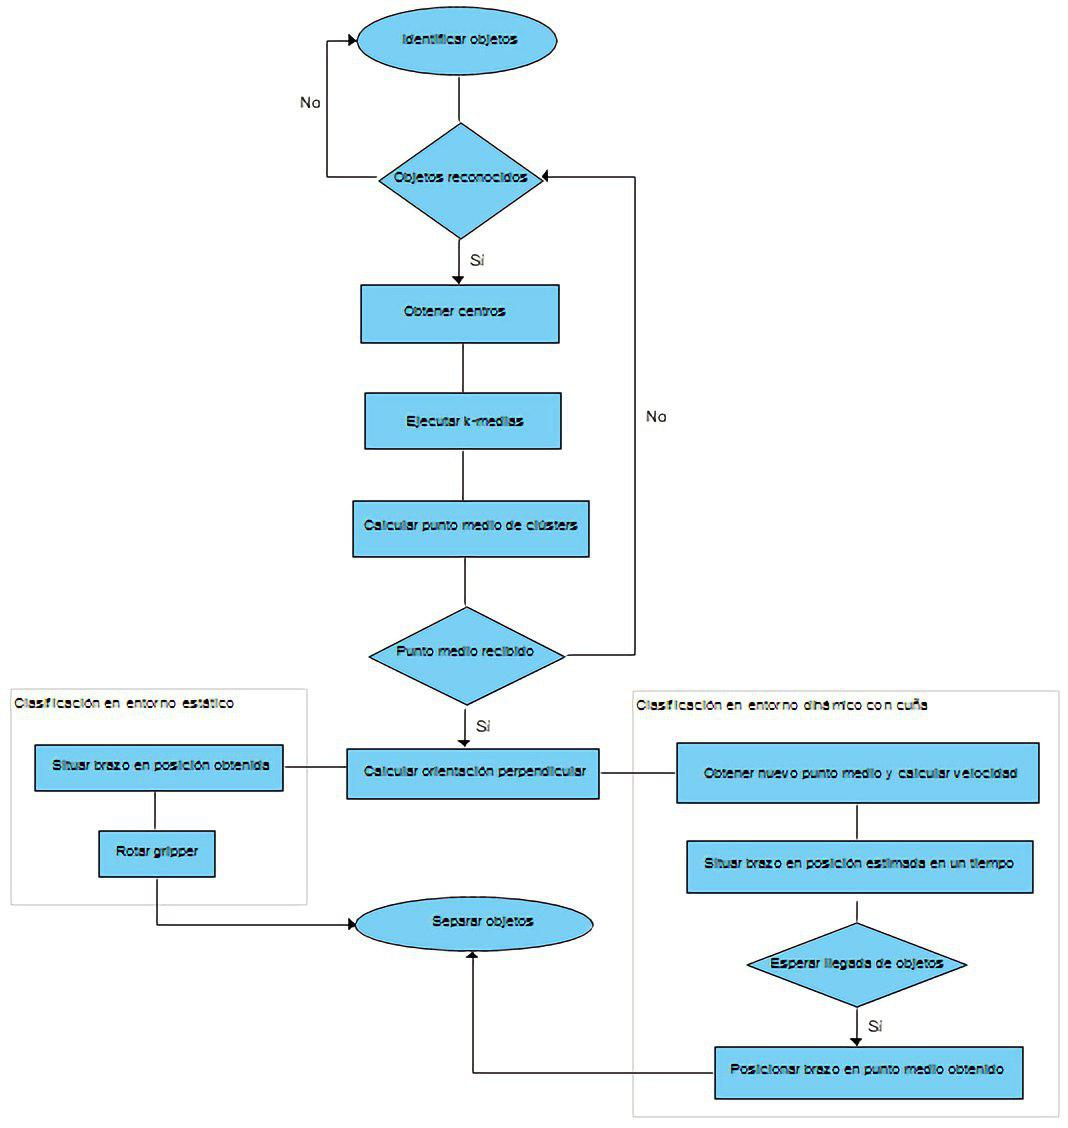
\includegraphics[scale=0.5]{imagenes/flowd.jpg}
	\caption{Diagrama de flujo.}
\end{figure}

\begin{itemize}
	\item \textbf{Módulo de reconocimiento.} Este es el que se encargará de identificar los objetos, procesar los datos y enviarlos al módulo de control de Baxter.\\
	\item \textbf{Módulo de control de Baxter.} La función de este módulo será realizar los movimientos y cálculos necesarios para separar los objetos. Además se incluye la planificación y ejecución de trayectorias. \\
\end{itemize}

\subsection{Módulo de reconocimiento}
\noindent Este módulo incorpora la visión por computador. Lo componen: \\

\begin{itemize}
	\item \textit{GetPosition}. Es la función encargada de obtener las coordenadas del centro de los objetos en la imagen.
	\item \textit{Get3DPos}. Se encarga de obtener las coordenadas en el mundo real a partir de las coordenadas de la imagen.
	\item \textit{GetRealPos}. A partir de las coordenadas dadas por \textit{Get3DPos}, obtiene el centro de los objetos en el mundo real.
	\item \textit{ImageCallBack}. Cada vez que se recibe una imagen, esta función se encarga de procesarla y enviar los datos a través de ROS al módulo de control de Baxter.
\end{itemize}

\subsection{Módulo de control de Baxter}
\noindent Como se dijo anteriormente, este es el módulo que se encargará del control sobre el robot, además de realizar algunos cálculos necesarios para poder clasificar los objetos. \\

\begin{itemize}
	\item \textit{baxter\_interface}: este nodo es el encargado de definir los brazos y \textit{grippers} de Baxter en Python. Para ello, se utilizan las siguientes órdenes: \\
	
	- \textit{right\_arm = baxter\_interface.limb.Limb('right')}
	
	- \textit{right\_gripper = baxter\_interface.Gripper('right')}\\
	
	Además, una vez se han definido los \textit{grippers}, estos se pueden calibrar y abrir o cerrar. \\
	
	
	\item \textit{moveit\_commander}: este es el nodo de MoveIt! para Python que se encargará de realizar los movimientos en Baxter y planificar la escena para detectar colisiones o utilizar RViz para moverlo. \\
	
	- \textit{p = PlanningSceneInterface(``base")}. Esta orden inicializa la escena en MoveIt!.\\
	- \textit{arms\_group = MoveGroupInterface(``both\_arms", "base")}. Se encarga de inicializar ambos brazos en la escena. \\
	- \textit{rightarm\_group = MoveGroupInterface(``right\_arm'', ``base")}. Inicializa el brazo derecho en la escena. Se realiza análogamente para el izquierdo.\\
	- \textit{rightarm\_group.moveToPose \\(position, ``right\_gripper'', max\_velocity\_scaling\_factor=1, plan\_only=False)}. Esta orden es la encargada de realizar los movimientos, en este caso, el brazo derecho se moverá hasta la posición ``\textit{position}'' con una velocidad máxima de 1 m/s. \\
	
	\item \textit{rotate\_pose\_by\_euler\_angles}: es la función encargada de rotar los \textit{grippers} a la orientación establecida.\\
\end{itemize}

\newpage
\section{Implementación}
\noindent Las tareas realizadas pueden clasificarse en tareas de visión por computador y tareas de control. En este apartado se explicará cada una de ellas, incluyendo todos los programas realizados a lo largo del proyecto. \\

\noindent Los tópicos de ROS realizan una tarea importante en este trabajo, ya que gracias a ellos podemos escribir códigos en distintos lenguajes de programación, en este caso, la visión en C++ y el control en Python, y compartir información entre ellos. A continuación se explica cada una de estas tareas. \\

\textbf{baxter\_img.cpp} Este código escrito en lenguaje C++ es el encargado del procesamiento de imágenes utilizando OpenCV y de enviar la posición del punto medio entre los dos clústers al tópico \textit{/classification}.\\

\textbf{pick\_and\_place.py} Este programa se subscribe al tópico \textit{/detected\_objects} para obtener la posición de los objetos y construir una torre con ellos. \\

\textbf{classif.py} Este archivo en Python se subscribe al tópico \textit{/classification} y realiza una clasificación de los objetos situados en la mesa. \\

\textbf{dyn\_classif.py} Este otro programa también escrito en Python se subscribe al tópico \textit{/classification} para realizar una clasificación en entorno dinámico con una paleta como herramienta. \\

\textbf{dyn\_wedge.py} Este último programa en Python obtiene el punto medio a través del tópico \textit{/classification} y realiza una clasificación en entorno dinámico con una cuña como herramienta.\\

\textbf{archivo.launch} Estos archivos son los encargados de inicializar el nodo de MoveIt! y RViz, la cámara del brazo derecho de Baxter y los programas de visión y control de cada caso definido anteriormente. \\ 

\textbf{CMakeLists.txt} Archivo que incluye los paquetes, dependencias y librerías que requiere el proyecto. \\

\textbf{package.xml} Define las dependencias de compilación y ejecución que requiere el proyecto además de definir algunas variables como el nombre, la versión o la licencia. \\

\subsection{Esquema general del escenario}
\noindent En este apartado se muestran los componentes utilizados en el escenario y las conexiones que se establecen entre ellos. \\

\begin{itemize}
	\item Objetos a clasificar. Se utilizarán varios objetos de distinto tamaño y color. Además se realizarán tests utilizando mayor o menor número de piezas. \\
	\item Cinta transportadora. Es la mesa sobre la que se posicionan los objetos. Se utilizará tanto en entorno dinámico como en estático. Para realizar la segmentación en entorno dinámico, se utilizarán las primeras velocidades de la cinta, que se pueden regular mediante la rueda de la que dispone la cinta. \\
	\item Baxter. Se utilizará el brazo robótico derecho para el control y la cámara de este mismo brazo para capturar las imágenes.\\
	\item Ordenador. Sobre este PC se ejecuta la versión de ROS acorde con la distribución de Ubuntu utilizada, en nuestro caso, ROS Kinetic. Este ordenador se conecta a través de una red Ethernet a Baxter y, mediante línea de comandos en un terminal RSDK, se comunica con él. \\
	
\end{itemize}

\begin{figure}[H]
	\centering % si queremos la imagen centrada
	\label{fig:esquema}
	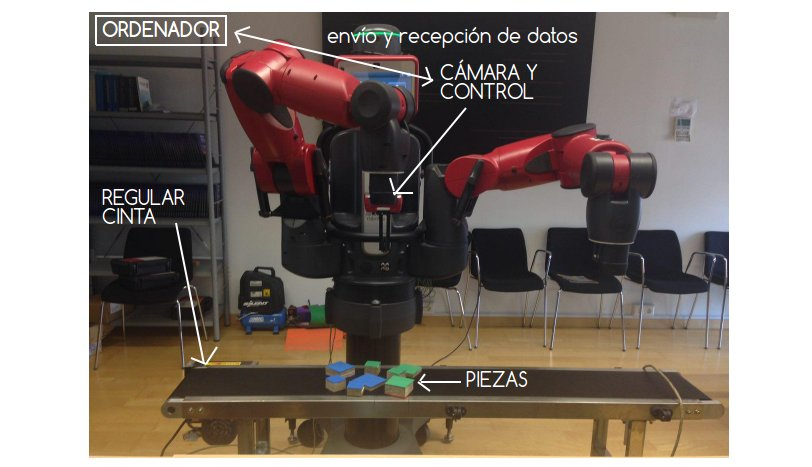
\includegraphics[scale=0.45]{imagenes/esquema.jpg}
	\caption{Esquema general del escenario.}
\end{figure}

\subsection{Visión por computador}
\noindent Como base para realizar la visión se ha utilizado un filtro de color \cite{maik}, a partir del cual se realiza la clasificación de objetos por color y posición. \\
\noindent En esta sección se explicarán estas funciones, que se pueden dividir en reconocimiento de objetos y procesamiento de imágenes. \\

\subsubsection{Reconocimiento de objetos}
\noindent Utilizando los tópicos de ROS se obtiene la imagen captada por la cámara del brazo derecho de Baxter, a partir de la cual se puede operar utilizando una función de \textit{callback} si existe, es decir, la función que se ejecutará al suscribirse al tópico de la cámara. En este caso esa función existe y se llama \textit{ImageCallback}. \\
\noindent Una vez se ha suscrito, es necesario conocer el color de los objetos rectangulares para reconocer su posición, tamaño y orientación, ya que sólo detectará los colores predefinidos en el código. Esto se realiza en formato HSV, estableciendo un rango para cada color de forma que estos se puedan filtrar en la imagen dejando el fondo negro; se han elegido colores con valores HSV lo bastante diferentes como para poder reconocerlos fácilmente, el azul y el verde. \\

\noindent Para calcular estos valores HSV, se ha utilizado el archivo hsvThresholder.py \cite{thpy}, al que se le pasa la imagen captada por la cámara de Baxter, que se puede ejecutar con el comando: \\

\textit{python hsvThresholder.py image.jpg} \\

\noindent Para obtener estos valores, es recomendable lanzar el programa para más imagenes con distintas posiciones de los objetos y distina iluminación. Se realizan capturas de los objetos con la máxima y la mínima iluminación posible, obteniendo un rango de valores HSV para los que se reconoce ese color. \\

\noindent Una vez se han reconocido los objetos que presentan los colores predefinidos, se obtiene su centro y se realiza un interlineado por sus bordes. En la siguiente figura \ref{fig:capter} se muestran distintas piezas identificadas en la ventana de visualización. Como se dijo anteriormente, estos objetos se han buscado por color en la captura proporcionada por el tópico de la cámara del brazo derecho. Se han obtenido sus centros en coordenadas de imagen, a partir de los cuales se han definido sus perímetros mediante líneas de color negro. \\

\begin{figure}[H]
	\centering % si queremos la imagen centrada
	\label{fig:capt}
	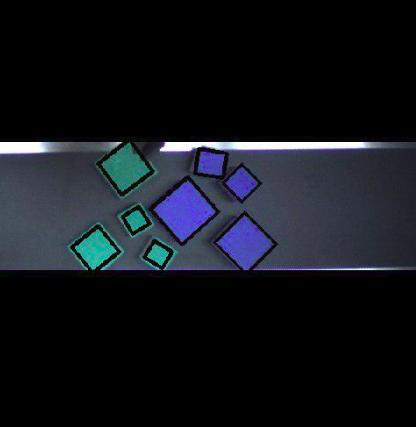
\includegraphics[scale=0.5]{imagenes/captura.jpg}
	\caption{Captura que muestra el reconocimiento de los objetos y la definición de sus perímetros.}
\end{figure}

\begin{figure}[H]
	\centering % si queremos la imagen centrada
	\label{fig:capter}
	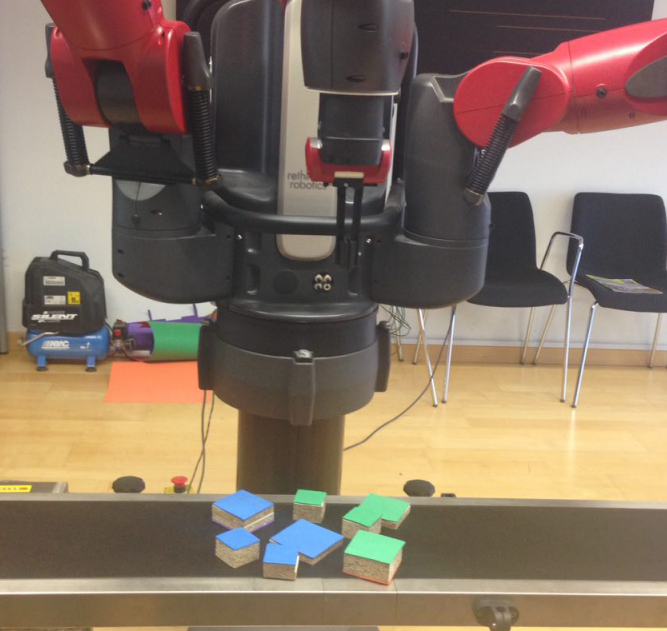
\includegraphics[scale=0.4]{imagenes/Baxter.png}
	\caption{Imagen que muestra la configuración de objetos de la imagen anterior \ref{fig:capt} desde fuera.}
\end{figure}

\subsubsection{Procesamiento de imágenes}
\noindent Al obtener la captura a través del tópico, se realiza una copia de esta a un tipo de dato correspondiente a una clase de OpenCV para imágenes, y se buscan, color por color, los objetos disponibles en esta imagen. \\

\noindent Para el posible ruido que pueda tener la imagen, se utiliza la función \textit{cvSmooth()} \cite{smooth} de OpenCV y se realiza un filtrado del rango de color que se está buscando en ese momento, dejando todo lo demás en negro. Se hace uso de la función \textit{cvErode()} \cite{erode} de OpenCV para borrar algunos puntitos blancos que pueden quedar tras filtrar la imagen. Tras esto, la imagen se pasa a escala de grises y se obtienen sólo los píxeles del objeto, logrando reconocer el rectángulo que lo define. El resultado de los objetos con el interlineado se muestra en una ventana de visualización (figura \ref{fig:capt}), por lo que el usuario puede determinar la calidad de detección de objetos con las características del entorno en el que se encuentra. \\

\noindent Una vez se ha conseguido obtener el centro de todos los objetos visibles en la imagen, se realiza el clustering con el algoritmo K-means (explicado en el anexo \ref{clustering}). Para ello, es imperativo el uso de un tipo de dato de OpenCV llamado \textit{Mat}, a través del que se copia un tipo de dato \textit{PoseArray}, un array de \textit{PoseStamped} que incluye las coordenadas de posición \textit{x, y, z} y las coordenadas de orientación, \textit{x, y, z, w}. Como se explicó en la sección de gestión de problemas (\ref{planif}), a través de este tipo de dato se le ha pasado tanto la posición del objeto como el color del mismo. \\
De la salida resultante del K-means se obtienen las etiquetas de cada uno de los objetos, siendo 0 si pertenece al clúster 0 y 1 si pertenece al 1, además de la posición obtenida en la última iteración de k-medias de los centroides que se han utilizado para obtener esos grupos, a partir de los que podemos calcular el punto medio y la orientación para realizar la clasificación. \\

\noindent Como todos estos cálculos se han realizado a partir de la imagen, las coordenadas que se han obtenido no nos valen para realizar las tareas de control, por ello, para enviar a través de un \textit{publisher} de ROS el valor del punto medio hay que realizar una conversión a coordenadas del mundo real, para lo que es necesario añadir desplazamientos, calculados empíricamente, a la conversión de las coordenadas \textit{x} e \textit{y} a coordenadas de la ``base'' de la escena de MoveIt!, ya que a la hora de realizar cualquier movimiento, este va a estar relacionado con la ``base'' en esta escena. \\

\subsection{Procedimientos de control}
\noindent Para la implementación de estas tareas se ha utilizado el lenguaje Python junto con el paquete \textit{moveit\_commander}, que permite realizar movimientos rectos con distinta orientación del \textit{gripper} o pinza. \\
\noindent Para realizar las tareas de clasificación, se han utilizado como herramientas una paleta y una cuña fabricadas a partir de cartón y goma eva, ya que las existentes, vistas en la sección \ref{chw}, no eran adecuadas para realizar este proyecto, puesto que se está trabajando con más de un objeto a la vez. \\

\subsubsection{\textit{Pick and place} adaptado}
\noindent Para este programa, se ha adaptado el código de \textit{pick and place} proporcionado por Gazebo. Gazebo \cite{gazebo} es un simulador de robots en 3D de código abierto que incluye una gran variedad de modelos y resulta bastante útil a la hora de realizar pruebas, diseñar o mejorar las implementaciones. Además permite crear un entorno acorde con el real y simular interacciones.\\
Esta implementación de la que se habla está destinada a ser ejecutada en este simulador. En este proyecto, como ejercicio de adaptación se ha utilizado este programa junto con visión por computador para realizar un \textit{pick and place} en el Baxter real (figura \ref{cd:pnp}).\\

\begin{figure}[H]
	\centering % si queremos la imagen centrada
	\label{cd:pnp}
	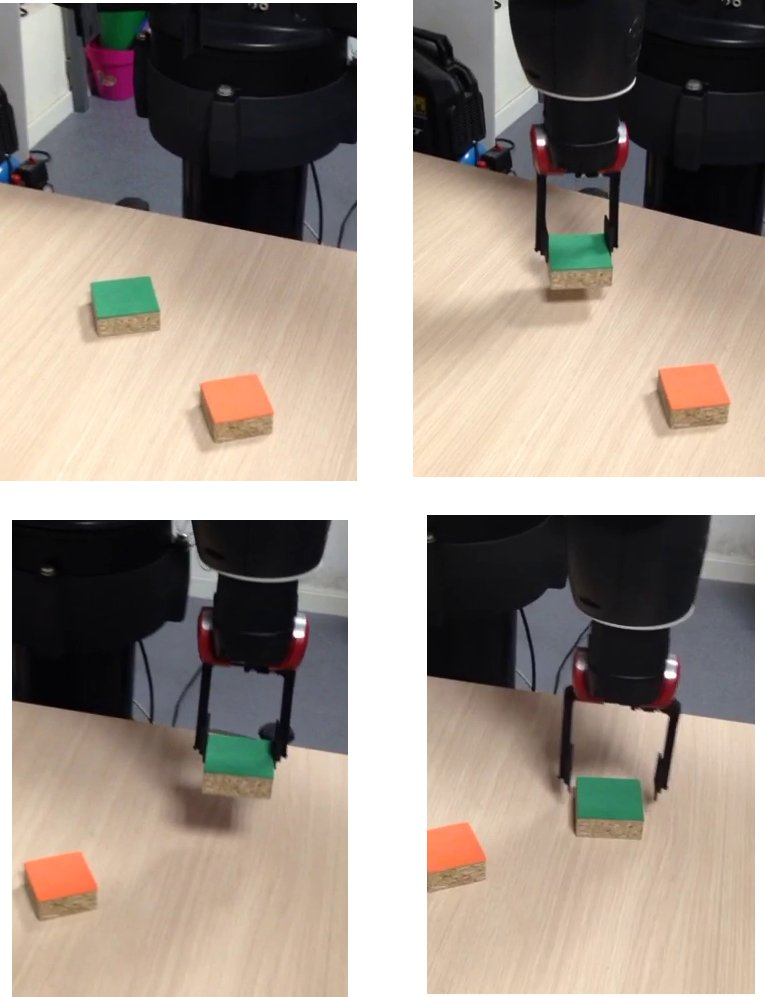
\includegraphics[scale=0.25]{imagenes/pandp.jpg}
	\caption{Capturas de la ejecución de \textit{pick and place} adaptado.}
\end{figure}

\subsubsection{Clasificación en entorno estático}
\noindent Conociendo el punto medio obtenido por el programa de visión, utilizando la paleta (figura \ref{cd:paleta}), Baxter mueve su brazo hasta esta posición con una orientación que también ha obtenido. Cuando se encuentra en esta posición, gira el \textit{gripper} hasta que forme 90º situándose en un eje horizontal y arrastra los objetos hacia arriba y hacia abajo, separándolos entre sí (figura \ref{cd:ce}). \\

\begin{figure}[H]
	\centering % si queremos la imagen centrada
	\label{cd:paleta}
	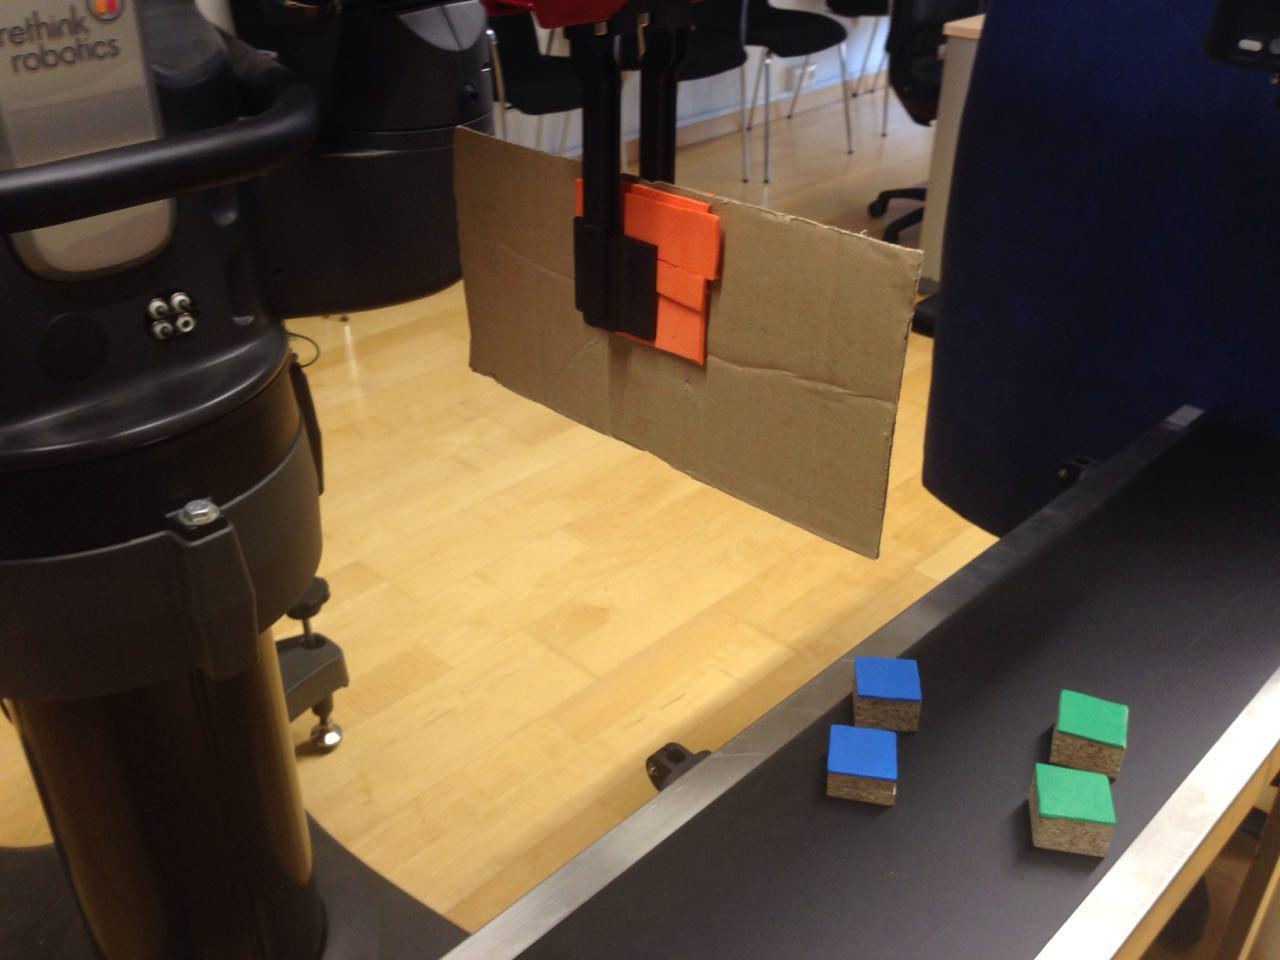
\includegraphics[scale=0.23]{imagenes/paleta.jpg}
	\caption{Paleta de cartón.}
\end{figure}

\begin{figure}[H]
	\centering % si queremos la imagen centrada
	\label{cd:ce}
	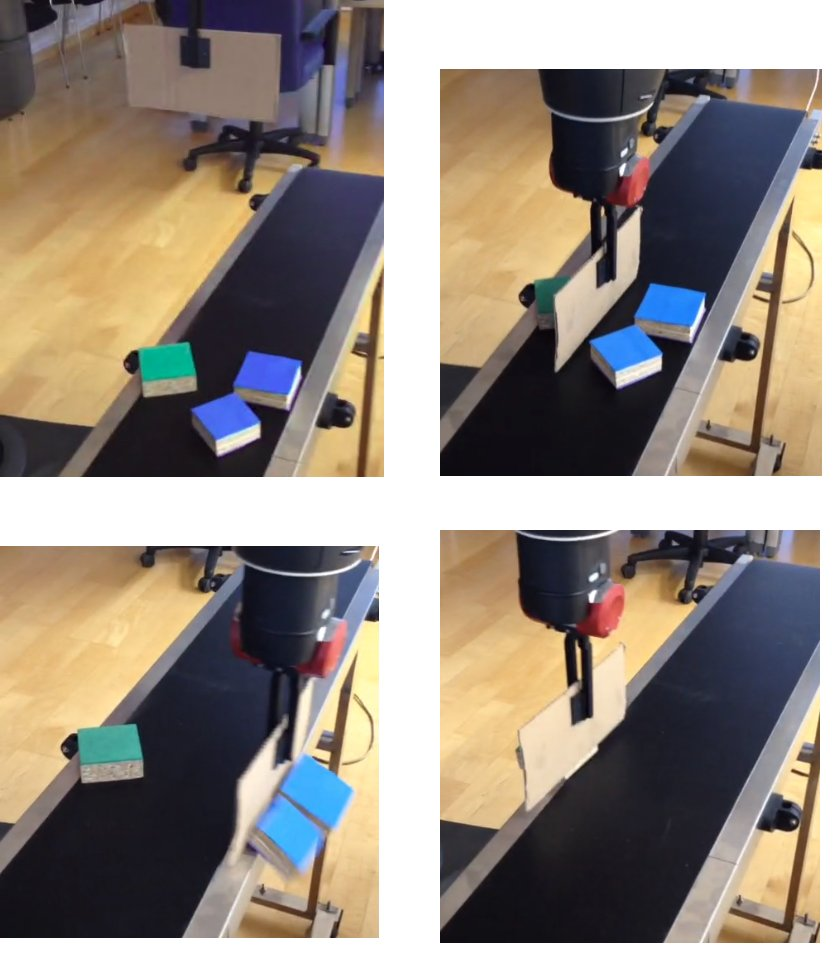
\includegraphics[scale=0.25]{imagenes/static.jpg}
	\caption{Capturas de la clasificación en entorno estático.}
\end{figure}

\subsubsection{Clasificación en entorno dinámico con cinta transportadora}
\noindent En este tipo de clasificación se han utilizado dos prototipos de herramienta, una cuña y una paleta hechas de cartón y goma eva para evitar el deslizamiento; sin embargo en una aplicación real, deberían utilizarse materiales más pesados y robustos, puesto que en ocasiones no se obtienen los resultados esperados debido al peso, rigidez o forma de estas sencillas herramientas construidas para la realización del proyecto. \\

\noindent El comienzo de ambas tareas es el mismo, obteniendo la posición en dos ocasiones separadas en el tiempo para conocer la velocidad y predecir en qué posición estarán en el momento de la separación. \\
\begin{enumerate}
	\item Clasificación utilizando como herramienta una paleta \ref{cd:paleta}\\
	
	Con esta herramienta se ha diseñado un comportamiento que separe primero los objetos de una clase y después los de la otra, calculando de nuevo la posición en la que se encontrarán entonces. \\ 
	Una vez conocemos la posición en la que estarán, el \textit{gripper} se sitúa en ese punto y espera a que los objetos lleguen, después separa en primer lugar los de abajo, apartándolos con la paleta en la dirección y con la orientación adecuadas. En ese momento además obtiene el punto en el que estarán situados los demás y al terminar de separar los anteriores va hacia esa posición, en la que realiza un movimiento análogo al realizado anteriormente pero en la dirección contraria (figura \ref{cd:pd}). \\
	
	\begin{figure}[H]
		\centering % si queremos la imagen centrada
		\label{cd:pd}
		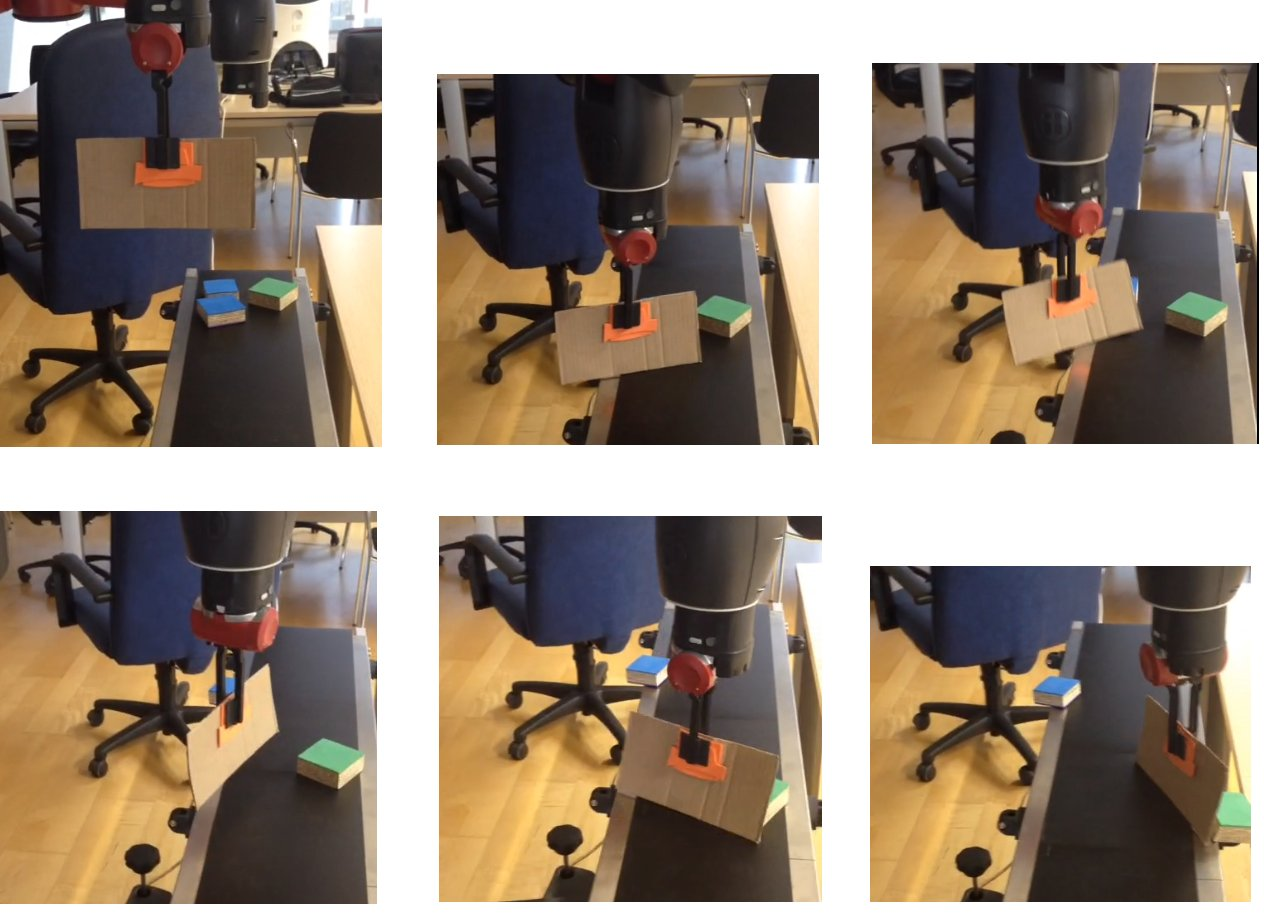
\includegraphics[scale=0.21]{imagenes/paletadyn.jpg}
		\caption{Capturas de la ejecución de la segmentación con paleta en entorno dinámico.}
	\end{figure}
	
	\item Clasificación utilizando como herramienta una cuña \\
	
	\begin{figure}[H]
		\centering % si queremos la imagen centrada
		\label{cd:cuna}
		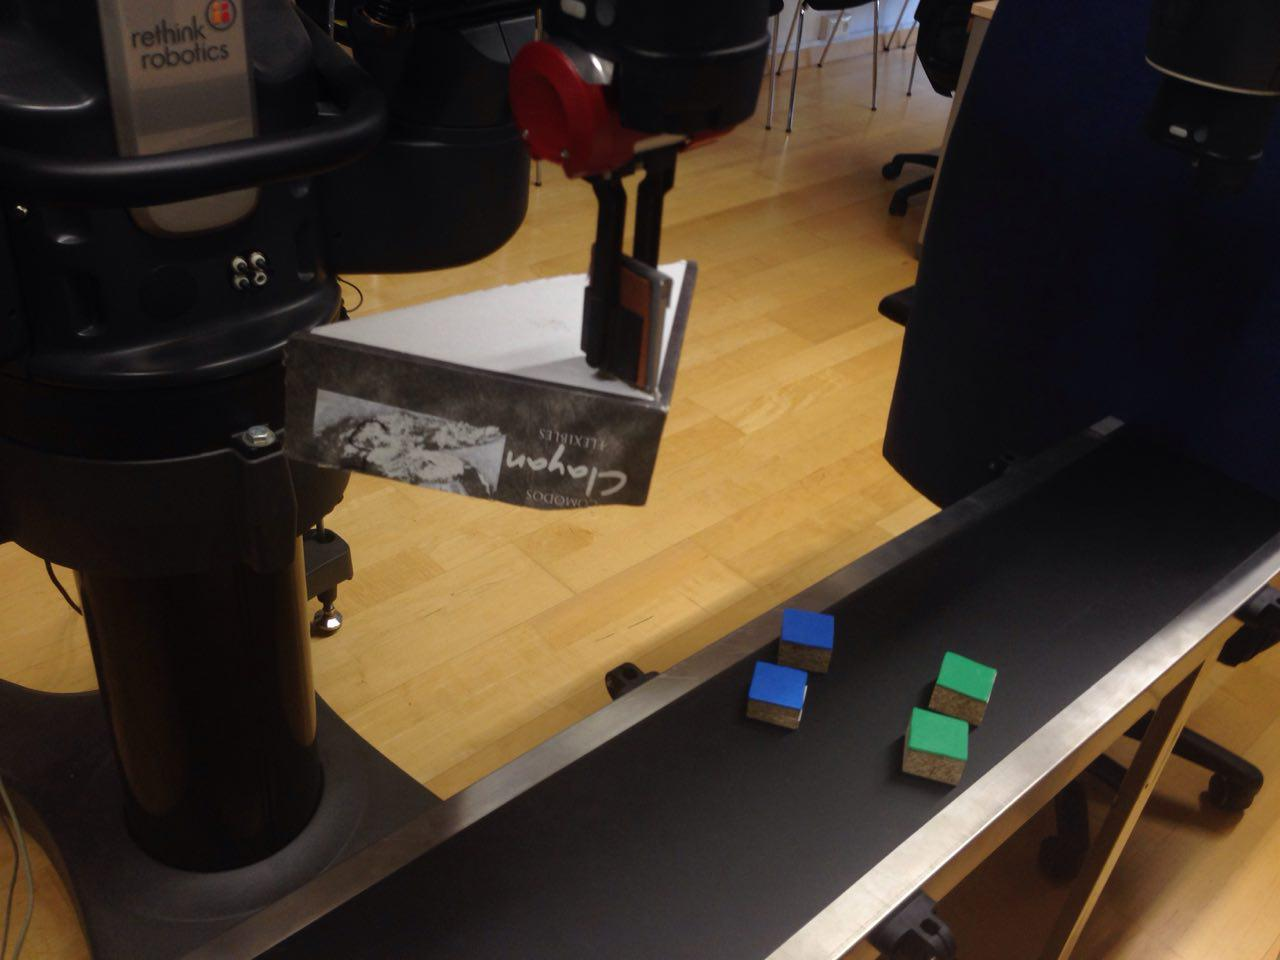
\includegraphics[scale=0.25]{imagenes/cunia.jpg}
		\caption{Cuña de cartón.}
	\end{figure}

	La cuña \ref{cd:cuna} es una herramienta que hace mucho más sencillo el control en este tipo de clasificación con cinta transportadora, por lo que las pruebas se realizarán con ella. Una vez se conoce la posición inicial, Baxter sitúa el brazo un poco más alejado de esta y con distinta orientación, de forma que pueda clasificar elementos cuya recta de separación tenga una pendiente más pronunciada. Cuando se detecta que los objetos han llegado a la posición en la que se encuentra la cuña, va hacia el punto que había calculado en un principio y avanza, de forma que los elementos se topen con los lados de la cuña y caigan fuera de la cinta transportadora, ayudándose de una oscilación en el eje vertical. (figura \ref{cd:cd})\\
	
	\begin{figure}[H]
		\centering % si queremos la imagen centrada
		\label{cd:cd}
		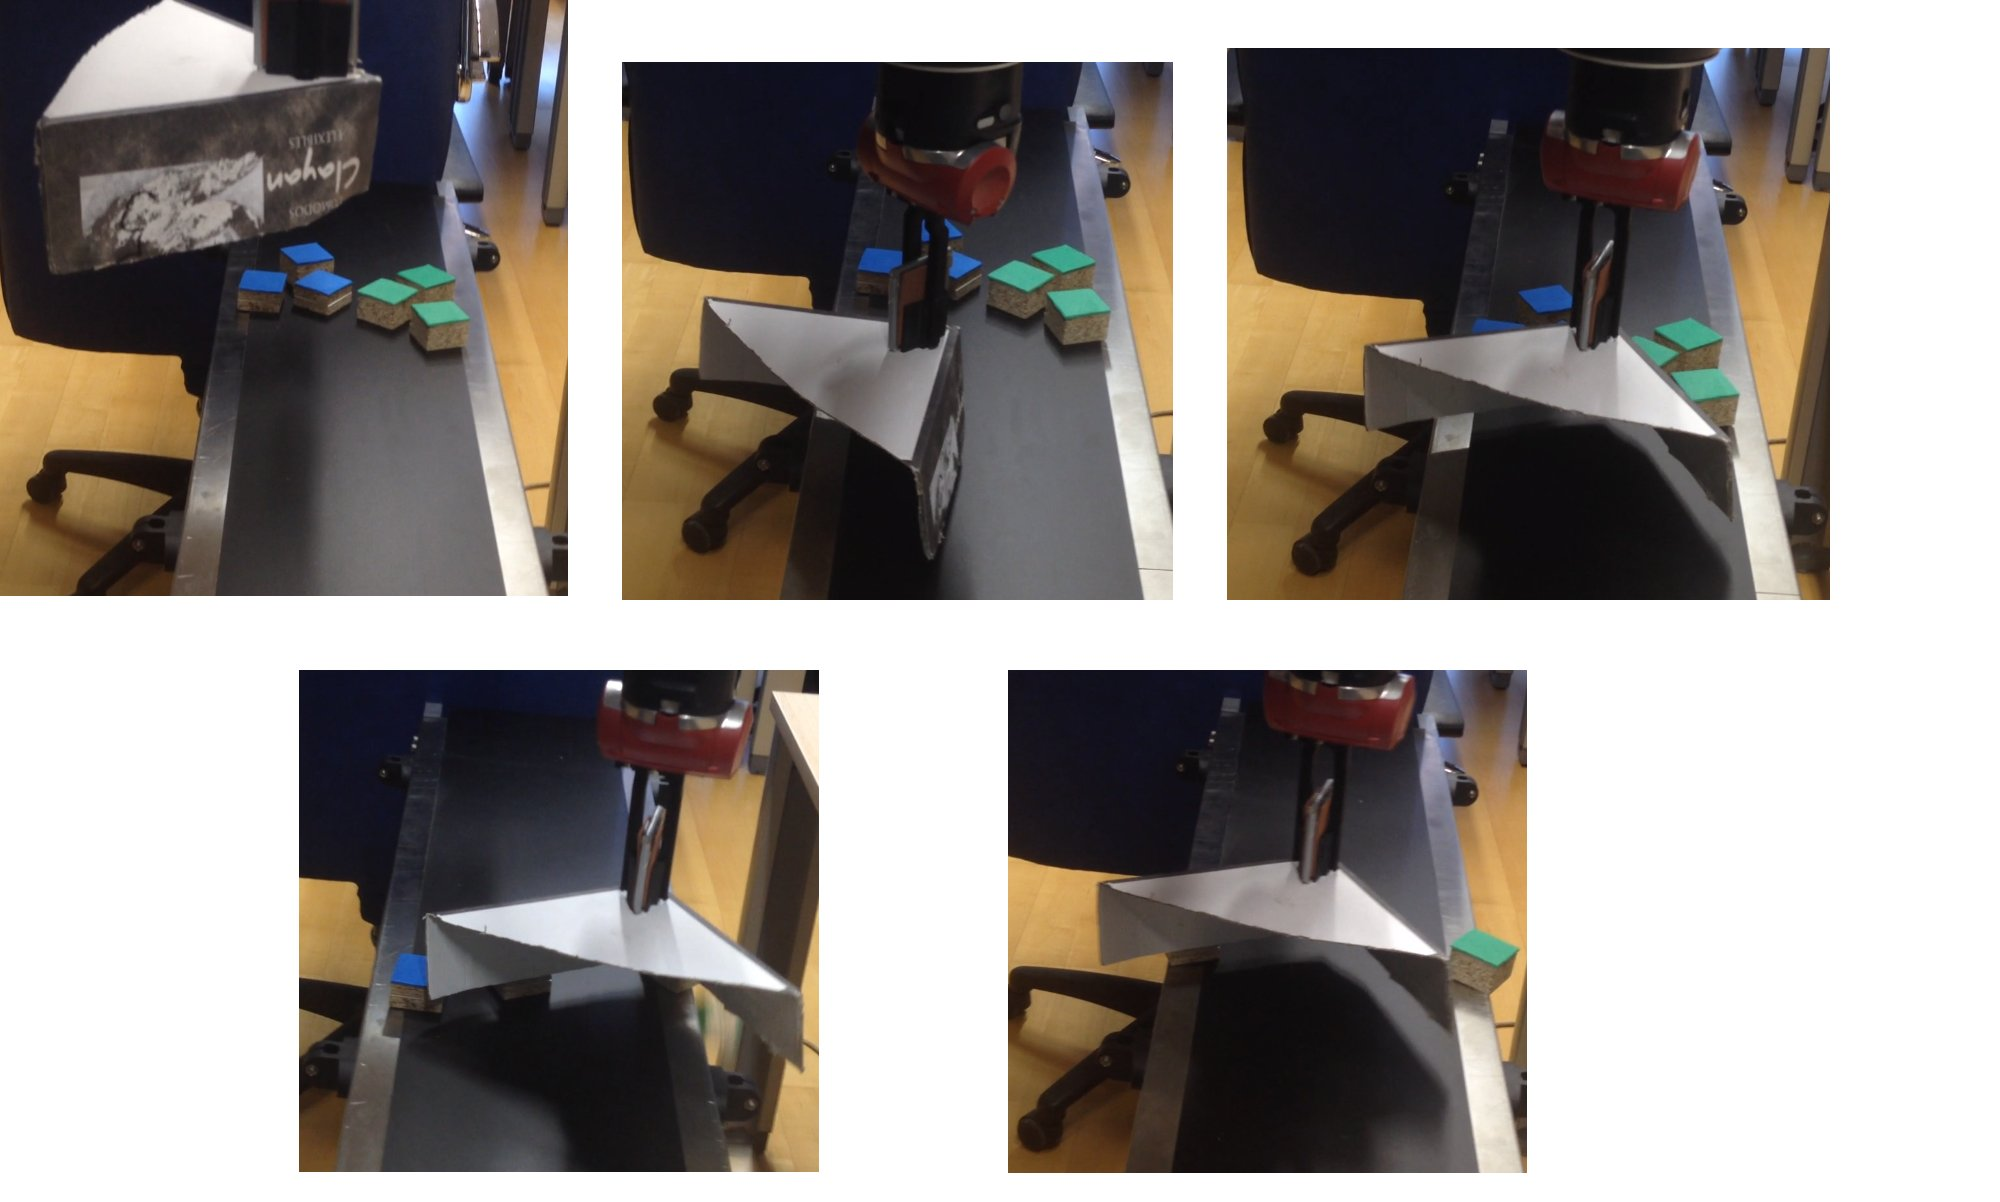
\includegraphics[scale=0.18]{imagenes/cunadyn.jpg}
		\caption{Capturas de la ejecución de la segmentación con cuña en entorno dinámico.}
	\end{figure}

\end{enumerate}
%
\newpage
\section{Pruebas}
\label{sec:pruebas}
\subsection{Introducción}
\noindent Para contrastar el funcionamiento de las tareas realizadas conforme a los objetivos fijados, se van a realizar una serie de pruebas para cada tipo de clasificación. \\

\section *{Métricas}
\noindent A continuación se exponen los experimentos realizados, así como la característica medida.

\begin{itemize}
	\item Medidas de rendimiento.
		\begin{itemize}
			\item Precisión frente a velocidad en clasificación dinámica.
			\item Precisión frente a exhaustividad en clasificación estática con misma configuración de objetos.
			\item Obtención del valor F para los valores de precisión y exhaustividad nombrados en el punto anterior.
			\item Precisión en robótica adaptativa.
		\end{itemize}
	\item Medidas de error. Estas se realizan tanto en entorno estático como dinámico.
		\begin{itemize}
			\item Precisión frente a número de objetos.
			\item Precisión frente a tamaño de objetos.
		\end{itemize}
\end{itemize}

	%\item Tiempo que tarda la clasificación estática frente a la dinámica.
	


\section*{Resultados}
\subsection{Medidas de rendimiento}
\noindent A continuación se muestran los resultados obtenidos para las pruebas de rendimiento. \\
\subsubsection{Precisión frente a velocidad en clasificación dinámica}
\noindent Para esta prueba, se han realizado unas 25 ejecuciones con distintas configuraciones (posición que toma cada objeto). Como vemos en la gráfica \ref{cd:ve}, cuanto mayor es la velocidad, menor es la precisión que se obtiene.\\

\begin{figure}[H]
	\centering % si queremos la imagen centrada
	\label{cd:ve}
	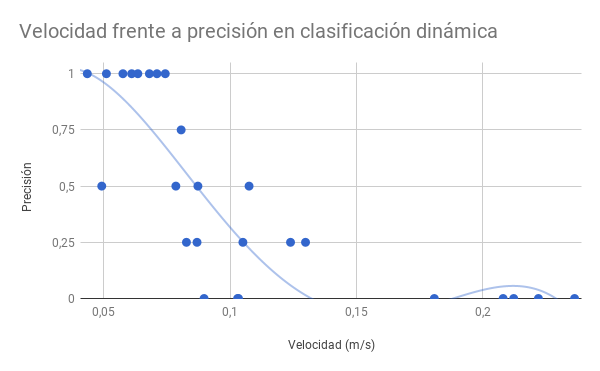
\includegraphics[scale=0.55]{imagenes/vel-eficiencia.png}
	\caption{Gráfica que muestra la velocidad frente a la eficiencia en clasificación dinámica con cuña donde la línea sigue un ajuste polinómico de grado 6.}
\end{figure}

%\begin{figure}[H]
%	\centering % si queremos la imagen centrada
%	\label{cd:areave}
%	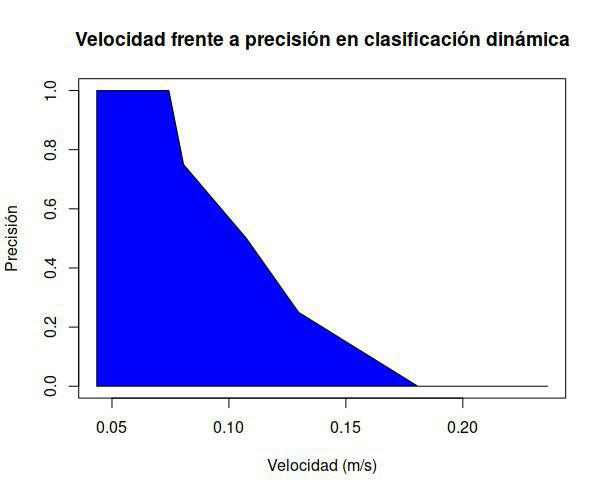
\includegraphics[scale=0.55]{imagenes/areave.jpg}
%	\caption{Gráfica que muestra la curva seguida por la velocidad frente a la precisión en clasificación dinámica con cuña}
%\end{figure}

\noindent Se ha realizado un ajuste de los datos obtenidos con una línea de tendencia de tipo polinómica de grado 4 y se ha obtenido la figura anterior \ref{cd:ve}. Los resultados obtenidos siguen una curva lógica, siendo los valores de precisión más bajos cuanta más velocidad lleva la cinta transportadora. Es por esto por lo que las siguientes pruebas que se realicen en un entorno dinámico se ejecutarán con una velocidad menor a 0.1 m/s. Sin embargo, si nos fijamos en la gráfica \ref{cd:ve}, podemos observar algunos puntos algo dispares con respecto a la media; esto puede deberse al algoritmo de planificación de MoveIt! utilizado, como se explicaba en la sección \ref{planif}. \\

\subsubsection{Precisión y exhaustividad}
\noindent Estos valores, utilizados en medicina como especificidad, \textit{``specificity''} y sensitividad, \textit{``sensitivity''} \cite{powers2011evaluation}, también pueden ser de ayuda a la hora de comparar un algoritmo de clasificación con otro. Para explicarlos, se va a mostrar un ejemplo tras definir estos conceptos.  \cite{pr} \\

\noindent A la hora de realizar una clasificación, se denomina al trabajo realizado de 4 posibles maneras fijándonos en el número de objetos verdes: \\

\begin{itemize}
	\item \textbf{Verdadero positivo}. En esta prueba, son aquellos objetos verdes que Baxter ha separado y que realmente eran verdes.
	\item \textbf{Verdadero negativo}. Son los objetos separados como verdes, pero que realmente son azules.
	\item \textbf{Falso positivo}. Son aquellos objetos azules que no se han separado.
	\item \textbf{Falso negativo}. Son los objetos verdes que han quedado por separar. \\
\end{itemize}

\noindent El valor de precisión, ``precision'', se refiere a los objetos clasificados como positivos que realmente son verdaderos positivos, mientras que la exhaustividad o ``recall'' es el ratio de verdaderos positivos. \\
\noindent Así, si tenemos un conjunto de 4 objetos verdes y 4 azules \ref{cd:clasif} y separamos 2 verdes y 1 azul, la precisión será 2/3 y la exhaustividad 2/4. Es decir, habremos separado únicamente 2 objetos que realmente son verdes de 4 objetos verdes que había en total. \\

\begin{figure}[H]
	\centering
	\label{cd:clasif}
	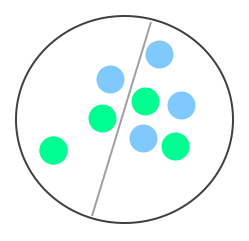
\includegraphics[scale=0.55]{imagenes/clasif.png}
	\caption{Ejemplo de precisión y exhaustividad en el que se ven los objetos que toma como verdaderos positivos (a la izquierda) y los que toma como negativos (a la derecha).}
\end{figure}

\noindent Para esta prueba, se ha realizado una modificación en el programa de clasificación estática, de forma que se pueda cambiar un parámetro ``\textit{precision}'' que permita separar en mayor o menor porcentaje el número de objetos de un color, de manera que se pueda medir la precisión y exhaustividad que se obtienen para unos valores predefinidos. \\

\noindent Se han realizado ejecuciones para valores del parámetro ``\textit{precision}'' de 0.5, 0.7 y 0.9 con 3 objetos de cada color, verde y azul. A continuación se muestra la gráfica de curvas PR, que consiste en una compensación entre precisión y exhaustividad para un diferente umbral, en este caso, el parámetro ``\textit{precision}''.\\

\begin{figure}[H]
	\centering
	\label{cd:pr}
	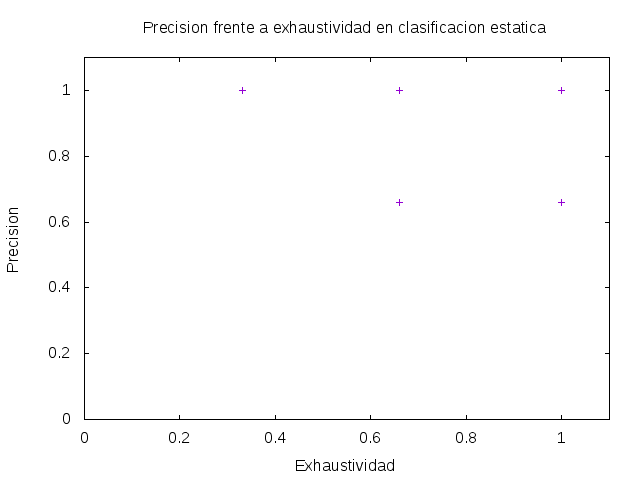
\includegraphics[scale=0.55]{imagenes/PR2.png}
	\caption{Gráfica que muestra la exhaustividad frente a la precisión en clasificación estática}
\end{figure}

%\noindent Para realizar el ajuste, se ha utilizado una línea de tendencia polinómica de grado 6. En este caso, los datos no son lo suficientemente significativos como para realizar esta curva, no existe ninguna función que siga los puntos obtenidos, esta es la mejor aproximación que se puede obtener. \\
\noindent El número de objetos de los que se dispone es de 3 de cada color, por lo que los valores de precisión y exhaustividad únicamente son 0.33, 0.66 y 0.99, ya que se obtienen en función del número de objetos verdes separados. No se ha realizado ninguna curva de ajuste ya que con los únicos datos que se pueden obtener no existe ninguna función que pueda aproximarse a ellos. \\

\noindent La alta precisión observada en la gráfica indica un bajo ratio de falsos positivos, mientras que un valor alto de exhaustividad indica un bajo ratio de falsos negativos \cite{scikit-learn}. En nuestro caso, la gráfica presenta valores altos para precisión y exhaustividad, por lo que se puede decir que los resultados son positivos, obteniendo una alta eficacia para los objetos clasificados. \\

\noindent Otra medida recurrente en este tipo de curvas consiste en calcular el valor F \cite{powers2011evaluation}, equivalente a la media armónica. Este valor une las dos medidas, precisión y exhaustividad, cuando sus valores son cercanos, de forma que podamos realizar comparativas de algoritmos con una sola variable. Su fórmula cuando la importancia que se le da a ambas medidas es la misma, es la siguiente: \\

%\centering
$ F_{1} = 2 * (precision * exhaustividad)/(precision + exhaustividad) $ \\

\noindent En caso de que no se le dé el mismo peso a ambas medidas se utiliza la siguiente fórmula: \\

$ F_{\beta} = (1 + \beta^{2}) * (precision/exhaustividad) / (\beta^{2} * precision + exhaustividad)$ \\

\noindent Ya que es una medida ponderada, en esta prueba se utilizará F2, una variante en la que se da más peso a la exhaustividad frente a la precisión, es decir, en nuestro caso, se intenta que se separe el mayor número de objetos verdes, aunque además se clasifique alguno azul con estos. La fórmula para ello es la siguiente: \\

$ F_{2} = 5 * (precision * exhaustividad)/(4* precision + exhaustividad) $ \\

\noindent Calculándolo para cada uno de los valores obtenidos en precisión y exhaustividad y quedándonos con el valor más alto se obtiene: $ F2 = 1 $, seguido de $ F2 = 0.9066 $.\\ 

\noindent Puesto que este valor es la media de ambas medidas precisión y exhaustividad, podemos decir que, como se explicó anteriormente, las pruebas realizadas para este número de objetos presentan una alta eficacia, separándose el mayor número de verdes posible. \\

\subsubsection{Robótica adaptativa}
\noindent Para esta implementación, se ha utilizado el código de clasificación en entorno estático. A partir de este, se ha definido una variable booleana que indica cuándo la segmentación se debe enfocar de forma adaptativa. Cuando esta variable se establece como \textit{True}, el programa preguntará la precisión obtenida en la ejecución anterior en un rango de [0:1] y la guardará en una variable. Como caso inicial, esta se debe establecer a -1. \\

\noindent A partir de este parámetro modificado a través de línea de comandos que llamaremos \textit{``precision\_value''} y otro valor \textit{alpha} inicializado a 0.1, el programa se encarga de alterar el valor de la coordenada \textit{x}, que en el caso de Baxter corresponde a la coordenada en el eje de ordenadas. De esta forma, cuanto menor sea el valor de \textit{``precision\_value''}, mayor será la modificación de la coordenada \textit{x}, que hará que el brazo de Baxter se sitúe más arriba, alcanzando más objetos de un mismo color. \\

\noindent Para mostrar el funcionamiento de esta aproximación se expone una tabla a partir de algunos resultados obtenidos, que consta del valor de precisión ``\textit{precision\_value}'' que se le proporciona en cada ejecución y de la precisión que realmente se obtiene. Se han utilizado 6 objetos, 3 de cada color, por lo que los valores de precisión que se pueden obtener son únicamente 0, 0.33, 0.66 y 1.

\begin{table}[H]
	\centering
	\begin{tabular}{|p{4cm} | p{4cm} |}
		\hline
		\textbf{\textit{precision\_value}} & \textbf{Precisión obtenida} \\ 
		\hline
		-1.0 & 1.0 \\
		\hline
		-1.0 & 0.66 \\
		\hline
		0.66 & 1.0 \\
		\hline
		0.66 & 0.66 \\
		\hline
		0.33 & 1.0 \\
		\hline
		0.0 & 1.0 \\
		\hline
		0.0 & 0.66 \\
		\hline
	\end{tabular}
	\caption{Tabla que muestra la precisión que se le indica al programa en cada ejecución y la precisión obtenida realmente.}
	\label{cuad:radap}
\end{table}

\noindent Al constar de pocos objetos, es difícil ver si realmente se ha mejorado la precisión. En la tabla se han incluido todas las combinaciones de resultados obtenidas en las 20 pruebas realizadas y, como se puede ver, cuanto menor es el valor que se le proporciona, mayor es la alteración de la coordenada \textit{x}, de manera que se mejore más eficazmente la precisión que se obtenga. \\

\subsection{Medidas de error}
\noindent Estas pruebas se han realizado tanto en clasificación dinámica como en estática. Es necesario tener en cuenta el tamaño de la cinta transportadora, ya que esta es bastante estrecha y no caben muchos objetos, de esta forma, se han realizado las ejecuciones para 4, 6 y 7 objetos de distinto tamaño.\\

\subsubsection{Clasificación estática}
\noindent Veremos primero los resultados obtenidos con objetos grandes y a continuación con objetos pequeños. \\
\begin{itemize}
	\item \textbf{Objetos grandes} \\
	\noindent En primer lugar, vemos la gráfica obtenida para configuraciones de objetos grandes de 4, 6 y 7 unidades. \\
	\begin{figure}[H]
		\centering % si queremos la imagen centrada
		\label{cd:eg}
		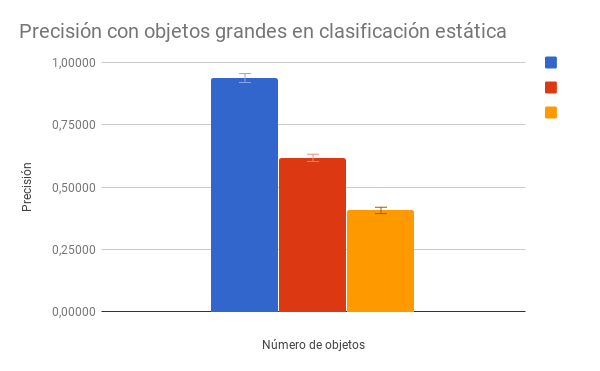
\includegraphics[scale=0.55]{imagenes/errbar_eg.png}
		\caption{Gráfica que muestra el número de objetos grandes frente a la precisión en clasificación estática, representando la media con una columna y la desviación típica con una barra.}
	\end{figure}

	\noindent En esta gráfica, se ha representado con un punto la media de los valores de precisión obtenidos en las ejecuciones para 4, 6 y 7 objetos, a la que se ha añadido una barra de error equivalente a la desviación estándar para el conjunto de resultados obtenidos con ese número de objetos. En este caso, no existe una gran variación de precisión en las ejecuciones, por lo que se ajusta bastante a la media. Como era de esperar, cuantos más objetos haya en la mesa, menos precisión se obtiene, puesto que la herramienta de la que se dispone no presenta la longitud adecuada para separar todos los objetos. \\
	
	\item \textbf{Objetos pequeños}
	\begin{figure}[H]
		\centering % si queremos la imagen centrada
		\label{cd:ep}
		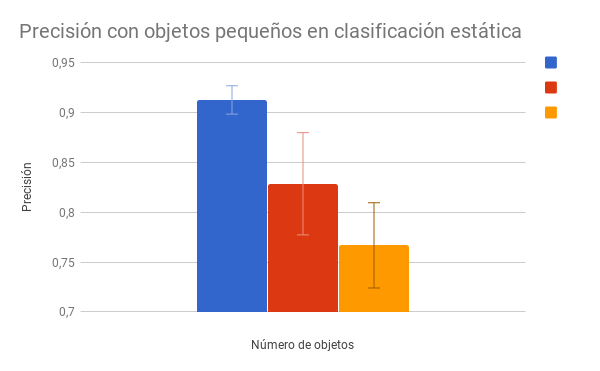
\includegraphics[scale=0.55]{imagenes/errbox_ep.png}
		\caption{Gráfica que muestra el número de objetos pequeños frente a la precisión en clasificación estática, representando la media con una columna y la desviación típica con una barra.}
	\end{figure}
	
	\noindent En este caso, vemos que la media de los valores obtenidos es bastante alta para las 3 configuraciones, ya que al ser más pequeños, la herramienta que en este caso lleva Baxter alcanza a la mayoría de ellos; si nos fijamos en la barra de error, para la configuración de 6 y de 7 objetos es más amplia, por lo que sabemos que ha habido más ejecuciones en las que no se han separado todos los objetos de un mismo color. \\
	
\end{itemize}

\subsubsection{Clasificación dinámica}
\noindent Del mismo modo que en la anterior, veremos primero los resultados con objetos grandes y después con pequeños, esta vez para clasificación en entorno dinámico utilizando una cuña como herramienta. \\

\begin{itemize}
	\item \textbf{Objetos grandes}

	\begin{figure}[H]
		\centering % si queremos la imagen centrada
		\label{cd:dg}
		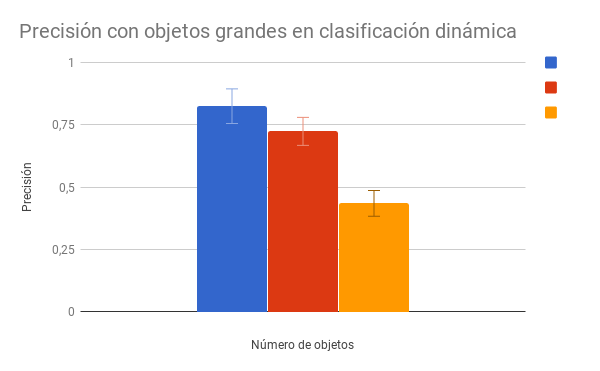
\includegraphics[scale=0.55]{imagenes/errbar_dg.png}
		\caption{Gráfica que muestra el número de objetos grandes frente a la precisión en clasificación dinámica con cuña, representando la media con una columna y la desviación típica con una barra.}
	\end{figure}

	\noindent Como muestra la figura, los resultados son bastante parecidos a los que nos encontramos en clasificación estática, aunque en este caso la barra de error o desviación estándar vuelve a ser más amplia. Esto se debe a que los objetos son grandes y de madera, Baxter sujeta la cuña de cartón con el \textit{gripper}, por lo que en algunas ocasiones el peso de los objetos vence la fuerza del \textit{gripper}, del que se resbala la cuña.\\

	\item \textbf{Objetos pequeños}
	
	\begin{figure}[H]
		\centering % si queremos la imagen centrada
		\label{cd:dp}
		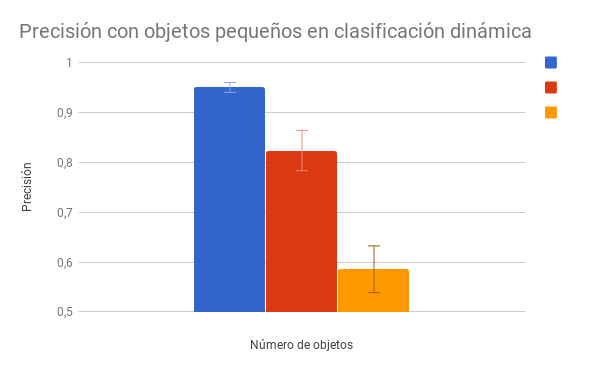
\includegraphics[scale=0.55]{imagenes/errbar_dp.png}
		\caption{Gráfica que muestra el número de objetos pequeños frente a la precisión en clasificación dinámica con cuña, representando la media con una columna y la desviación típica con una barra.}
	\end{figure}
	
	\noindent En la figura \ref{cd:dp} podemos ver que la utilización de objetos pequeños permite obtener mejores resultados en este entorno, ya que se consigue una eficiencia de casi 1 para 4 objetos, y para 6 y 7 no baja de 0.5. \\
	
\end{itemize} 

\noindent En definitiva, con los objetos pequeños se obtiene una mayor eficiencia en ambas clasificaciones, aunque esto se puede deber a las herramientas utilizadas, ya que no son las comunes que se utilizarían en una fábrica. Con las adecuadas se podrían obtener resultados preferentes a los mostrados en cuanto al peso o el área que ocupan en la mesa los objetos. \\
%
\newpage
\section{Conclusión}
\noindent Para concluir, se va a realizar una comparativa entre los objetivos fijados al principio del proyecto y los resultados logrados a lo largo de este. Finalmente, se describirán las capacidades adquiridas y algunos proyectos futuros que se proponen a partir del desarrollo de este. \\

\noindent La sección de Introducción (\ref{intro}) dio una visión general sobre los objetivos de este trabajo, en él se han utilizado herramientas como MoveIt!, los tópicos y servicios de ROS, y las librerías de OpenCV para implementar la visión por computador. \\
El objetivo principal de este proyecto (sección \ref{objetivos}) consistía en hacer que el robot Baxter clasificase objetos por color y posición en un entorno dinámico. Para lograrlo, se ha pasado por distintas fases ya nombradas anteriormente, como la adaptación de un programa de \textit{pick and place} del simulador Gazebo para la familiarización con el entorno, la clasificación de objetos en entorno estático y distintas posibilidades de realizar la segmentación en entorno dinámico. Así, con estos objetivos fijados se ha utilizado un desarrollo en espiral (sección \ref{software}) como metodología seguida para la planificación de tareas, lo que ha permitido mejorar continuamente el trabajo realizado. \\

\noindent Todos estos programas se han puesto a prueba, como veíamos en la sección \ref{sec:pruebas}, en la que se ha estudiado la precisión, velocidad y capacidad de procesamiento en estas funciones, por parte de Baxter y de las distintas herramientas nombradas. Además, se ha implementado un módulo de robótica adaptativa, que permite a Baxter realizar la mejor aproximación a partir de la precisión adquirida en la ejecución anterior. \\

\noindent En cuanto a los aspectos éticos, aunque en muchas ocasiones se piense que la automatización de tareas acaba con muchos puestos de trabajo, con las ventajas ya vistas en la sección \ref{actualidad}, resulta de gran interés el intentar que esas características idílicas generen beneficios a nuestro favor. \\

\noindent En general, los resultados obtenidos en este proyecto pueden resultar útiles para proyectos futuros; por ello, la implementación y el contenido de este trabajo será abierto y estará disponible en \textit{GitHub} \cite{crgh} y en la página web del laboratorio \cite{cvrlab}.

\subsection{Competencias adquiridas}
\noindent A lo largo de este proyecto, se han adquirido las siguientes capacidades:

\begin{itemize}
	\item \textbf{Familiarización con el entorno ROS.} ROS es un sistema operativo distribuido, en el que se ejecutan varios nodos en paralelo, controlados por tópicos, servicios y mensajes. En este proyecto se ha realizado un estudio de todos sus módulos a través de la documentación que proporciona para conseguir controlar el robot.
	\item \textbf{Librería OpenCV.} Esta es la librería utilizada en el módulo de visión por computador. Para la realización de este proyecto ha sido necesario el estudio de variables y funciones que esta librería proporciona.
	\item \textbf{MoveIt!.} Esta plataforma ha permitido realizar los movimientos correspondientes para separar los objetos. Gracias a su uso se han conseguido movimientos más rectos y simples que los que se conseguían con ROS. \\
\end{itemize}

\subsection{Trabajos futuros}
\noindent El resultado de las pruebas de este trabajo no se ha obtenido en su totalidad mediante código; al concluir una ejecución, sería una mejora significativa que Baxter pudiese autoevaluarse a sí mismo, conociendo los objetos que ha separado bien, los que no ha movido y los que ha clasificado mal. \\

\noindent Otra posible extensión de este trabajo consistiría en realizar un \textit{pick and place} en entorno dinámico. \\

\noindent Otra aproximación podría apoyarse en utilizar piezas de otros tamaños, formas y colores, quizás, realizando una clasificación en un entorno real con aceitunas o tomates, entre otras frutas y verduras. \\

\noindent La velocidad de la cinta transportadora podría regularse automáticamente, teniendo en cuenta la velocidad de ejecución de las trayectorias, de forma que se maximice la precisión de la clasificación de las piezas. \\

%
\newpage

\section{Anexo. Algoritmos de clustering}
\label{clustering}

\noindent En este anexo, se explicarán los algoritmos de clustering y, en concreto el algoritmo K-means \cite{hartigan1979algorithm}, que es el algoritmo utilizado en este proyecto. \\

\noindent El clustering es un método de aprendizaje no supervisado. La función de los algoritmos de clustering consiste en agrupar en conjuntos de datos una información. Dado un conjunto de datos, se utiliza un algoritmo de clustering para clasificar cada uno de los puntos en un grupo específico. Cada grupo contiene un grupo de objetos con características similares entre ellos. \\

\noindent Para este proyecto, se utiliza el algoritmo de clustering K-means.

\subsection{Algoritmo K-means}
\noindent El algoritmo K-means (K-Medias en español) consiste en un tipo de aprendizaje no supervisado, es decir, se ajusta a las observaciones sin conocer los datos. Este algoritmo se encarga de encontrar K clústers en los datos proporcionados, siendo K una entrada. 

\subsubsection{Cómo funciona}
\noindent Este algoritmo toma dos entradas, K (el número de clústers deseados) y un conjunto de datos. Para empezar, sitúa K centroides en posiciones aleatorias, y, para cada punto de la entrada encuentra el centroide más cercano y lo asigna al clúster perteneciente a ese centroide. Una vez están todos los puntos identificados y clasificados, para cada clúster se calcula un nuevo centroide que consistirá en la media de todos los puntos asignados a él, calculará de nuevo qué puntos pertenecen a esos clústers y parará cuando se mantengan los puntos incluidos en estos.

\subsubsection{Por qué elegir K-means}
\noindent Este algoritmo es de orden O(n). Es bastante rápido, ya que lo único que hace es calcular las distancias entre los puntos y clústers. \\
\noindent Una desventaja aparece a la hora de elegir el parámetro K, pues no siempre es trivial. Además, este algoritmo posiciona inicialmente dos centroides aleatoriamente, y esto puede llevar a obtener diferentes clasificaciones en varias ejecuciones con la misma configuración.\\

\noindent En nuestro caso conocemos el valor de K, puesto que disponemos de dos grupos de objetos. Además, se ha elegido este algoritmo por su simpleza y porque, en contraste con otros algoritmos de clustering, es el más rápido para estas tareas.
%
%%\chapter{Conclusiones y Trabajos Futuros}
%
%
%%\nocite{*}
%\bibliography{bibliografia/bibliografia.bib}\addcontentsline{toc}{chapter}{Bibliografía}
%\bibliographystyle{miunsrturl}
\newpage

\bibliography{bibliografia/bibliografia} 
\bibliographystyle{ieeetr}
%
%\appendix
%\input{apendices/manual_usuario/manual_usuario}
%%\input{apendices/paper/paper}
%\input{glosario/entradas_glosario}
% \addcontentsline{toc}{chapter}{Glosario}
% \printglossary

\chapter*{}
\thispagestyle{empty}

\end{document}
